%%This is a very basic article template.
%%There is just one section and two subsections.
\documentclass{article}

\usepackage{amsmath}
\usepackage{amscd}
\usepackage{amssymb}
\usepackage{amsfonts}
\usepackage{amsthm}
\usepackage{amsfonts}
\usepackage{amsthm}

\usepackage{circuitikz}
\usepackage{pgf}
\usepackage{tikz}
\usetikzlibrary{arrows,snakes,backgrounds}
% \usetikz
\usepackage{subfig}

\usepackage[super]{nth}
% \usepackage{appendix}
% \usepackage{listings}
% \usepackage{color}
\usepackage{ulem}
\usepackage{hyperref}
%\usepackage{url}
\usepackage{cancel}
\usepackage{cleveref}
 
\usepackage{aviolov_style}
\usepackage{local_style} 


\begin{document}


\title{Optimal Design for estimation in stochastic LIF models - \\ Mutual
<<<<<<< HEAD
Information + Maximum Principle / Dynamic Programing Approach} 
\author{Alexandre
Iolov, Susanne Ditlevsen, Andr\'e Longtin \\ $<$\href{mailto:aiolo040@uottawa.ca}
=======
Information + Dynamic Programing Approach} \author{Alexandre Iolov, Susanne
Ditlevsen, Andr\'e Longtin \\ $<$\href{mailto:aiolo040@uottawa.ca}
>>>>>>> 6d1ee3c9eb52b6bed66343a6488d0f9a4ca3aef0
		{aiolo040 at uottawa dot ca}$>$}

\date{\today}

\maketitle

\abstract{Given a stochastic differential equation with unknown parameters and a
control in the drift term - we discuss optimal design-type questions on what is
the best external perturbation in order to facilitate the estimation of the
unknown parameters} 

\tableofcontents 

\section{Problem Formulation}
The basic goal of 'Optimal Design' is to perturb a dynamical system in an
'optimal' way such as to 'best' estimate its structural parameters.

Consider the generic parametrized and controlled SDE system 
\begin{equation}
dX = U(x,\a(x,t); \th) \intd{t} + \sqrt{2D} dW
\label{eq:SDE_evolution} 
\end{equation}
and for illustration case also consider the simplest non-trivial example of
\cref{eq:SDE_evolution}, the OU system:
\begin{equation}
dX = \underbrace{(\a + \b( \mu - X)}_{U(x,\a; \th)} \intd{t} +
\underbrace{\s}_{\sqrt{2D}} dW
\label{eq:OU_evolution} 
\end{equation}
Whose parameter set is:
$$
\th = \{\m, \b, \s\}
$$
Sometimes, to make things simpler, we will assume that we know the diffusion
coefficient, $\s$, in which case the parameter set to-be-estimated for the OU
system becomes: 
$$
\th = \{\m, \b\}
$$ 

Out ultimate goal is to choose the control policy $\a(\cdot)$, such as to
facilitate the estimation of the parameter set $\th$ given a single observed
trajectory $\{X_t\}_0^T$. At first we will idealize that we have cts.
observations (i.e.\ very-high-frequency observations). Later we can try
addressing the problem of low-frequency observations. 

A fundamental concept in the sequel is the probabilty transition density
associated with $X_t$, we will call this $f$
\begin{equation}
f(x,t| x_0 ;\th, \a(\cdot)) dx = \Prob[ X_t \in x + dx | x_0, \a, \th]
\end{equation} 

It is well-known that for a fixed, $\th, \a(\cdot)$, $f$ is the solution to a
Fokker-Planck equation:
\begin{equation}
\di_t f = \L_{\th, \a(\cdot)}[f]
\label{eq:fokker_planck_forward_density}
\end{equation}
where the differential operator $\L$ is given by:
$$
\L_{\th, \a(\cdot)}[f] = D \cdot \di_x^2 [f] - \di_x[U(x,\a(x,t); \th) \cdot f]
$$
We will call $\L$ the forward operator and its adjoint $\Lstar$, the backward
operator.


\section{Optimal Design using Mutual Information}
Our main point-of-departure in obtaining $\a(\cdot)$ is the concept of Mutual
Information (here are two books on information theory -
\cite{Cover2006,MacKay2003}, see \cref{sec:mutual_info_defn} for definitions).

In particular, two references suggest that one should use the Mutual
Information \cite{Myung2013,Lewi2009} as the criterion for designing the
experiment. (Designing the experiment is synonymous to choosing the control policy
$\a(\cdot)$.

In order to apply the concept of mutual information, we need to have a prior on
the parameter set, $\th$. We will call this prior: 
$$\rho(\th).$$ 
Naturally a optimally-designed experiment is one which reveals most the actual
value of $\th$. That is we want to choose $\a(\cdot)$ such as to maximize the
Information in the random variable $\th$, given observations of the random
variable $X_t$.

First we need to consider the posterior of $\th$, $p(\th|X_t)$ given an
observation $X_t$ for $t$ fixed
\begin{subequations}
\begin{equation}
p(\th| X_t; \a) =
\frac{f(X_t,t|\th; \a)\cdot \rho(\th)}
{\int_\Theta f(X_t,t|\th; \a)\cdot \rho(\th)
\intd{\th}}
\label{eq:parameter_posterior_single_observation}
\end{equation} 
That is the transition density is the likelihood of the parameters.
\begin{equation}
L(X_t|\th ) = f(X_t, t| x_0, 0; \th, \a(\cdot))
\label{eq:paramter_likelihood_single_observation}
\end{equation}
\end{subequations}
However, if we have many observations $\{X_{t_n}\}$, the likelihood is, of
course, more complicated. Then 
\begin{subequations}
\begin{equation}
L(\{X_n\} | \th) = 
\prod_n (f(X_{t_{n+1}},t_{n+1}|X_{t_{n }},t_{n} ;\th)
\end{equation}
and the parameter posterior is then
\begin{equation}
p(\th| \{X_{t_n}\}; \a) =
\frac{L(\{X_{t_n}\},t|\th; \a)\cdot \rho(\th)}
{\int_\Theta L(\{X_{t_n}\},t|\th; \a)\cdot \rho(\th)
\intd{\th}}
\label{eq:parameter_posterior_multi_observations}
\end{equation}  
\end{subequations}
Once we have the concepts of the prior, posterior and likelihood, $\rho, p, L$,
then the mutual information, $I$, between the two random variables, $\th$, $X_t$
is: 
\begin{equation}
I(\a) = \int_\Theta \int_X  \log\left[\frac{p(\th| x; \a)}{\rho(\th)}\right]
\cdot L(x| \th;\a) \cdot \rho(\th) \intd{\th} \intd{x}
\label{eq:mutual_info_with_posterior}
\end{equation}
This is straight from equations 6,8,9 of \cite{Myung2013} (That paper is on the
OptEstimate Mendeley group). Also see \cref{sec:mutual_info_defn}.
 
Replacing the posterior in \cref{eq:mutual_info_with_posterior}, with the
bayesian formula from \cref{eq:parameter_posterior_single_observation} or
\ref{eq:parameter_posterior_multi_observations}, we get:
\begin{equation}
I(\a) = \int_\Theta \int_X  \log\left[\frac{L(x|\th; \a)}
										{\int_\Theta L(x|\th;\a)\cdot \rho(\th) \intd{\th}} \right] \cdot L(x|
										\th;\a) \cdot \rho(\th) \intd{\th} \intd{x}
\label{eq:mutual_info_with_likelihood}
\end{equation}

It is a small step then to seek the policy $\a(\cdot)$ that maximizes
$I$.

However \cref{eq:mutual_info_with_likelihood} can appear deceptively
simple. The integral over $X$, $\int_X \intd{x}$, is really a multi-dimensional integral
over all observations. Thus just the evaluation of $I$ is only possible through
Monte Carlo methods (unless there are very few,  say $N<5$ observations).
However if you have only one observation, as with the posterior given
\cref{eq:parameter_posterior_single_observation}, then we have a very simple
single integral over $x$, which can be easily evaluated approximately using any
quadrature rule.

A crucial assumption in the sequel is that we will NOT be updating the prior on
the fly, that is we will always have the same $\rho(\th)$ in
\cref{eq:mutual_info_with_likelihood}, even though new observations can
obviously be used to update the prior, $\rho$, through Bayes' formula.

\section{Finding the optimal design $\a(\cdot)$ - Dynamic Programing}
\label{sec:DP_4_OptEstimate}
In principle now, we have a criterion, the mutual information in
\cref{eq:mutual_info_with_likelihood}, using which to select the most
informative perturbation $\a(\cdot)$. 

However, in its most generality, $\a(\cdot)$ is a stochastic process measurable
wrt.\ the filtration of $X_t$. I.e.\ we will choose different control values
$\a(t)$ depending on the up-to $t$ realization of $X_s ; s\leq t$.

This is clearly a problem from optimal stochastic control. However, the
objective in \cref{eq:mutual_info_with_likelihood} is not in the form
needed to apply dynamic programing (or the maximum principle for that matter).
The multi-dimensional integral in $X$ makes things 'too' complicated. 

On the other hand, what we propose to do is to take the mutual information
criterion in \cref{eq:mutual_info_with_likelihood} using the single observation
likelihood in \cref{eq:paramter_likelihood_single_observation} and just integrate it over time.
\begin{equation}
J(\a)  = \int_\th \int_0^T\int_X
 \log\left(\frac{f(x,t|\th ; \a(\cdot) )}
 			{\int_\th f(x,t|\th; \a(\cdot)) \rho(\th)\intd{\th}}\right) 
 f(x,t|\th; \a(\cdot)) \cdot \rho(\th) \intd{x}\intd{t}\intd{\th}
\label{eq:mutual_info_time_integrated}
\end{equation}
where the $dx$ integral has the same dimension as the dimension of the SDE
not the dimension of the number of observations. I should repeat that $J$ is NOT
the mutual information between a realization of the process, $\{ X_t\}_0^T$ and
the parameter set, $\th$. It is the time-integral of the individual mutual
informations between each $X_t$ at time $t$ and the parameter set $\th$. The
reason we do this is that now $J$ can be written as
\begin{equation}
J( \a) = \Exp_{\th} \Bigg[
\Exp_{X_t|\th; \a(\cdot)}
\left[ \int_0^T \log\left(\frac{f(X_t,t|\th; \a(\cdot))}
{\int_\th f(X_t,t|\th; \a(\cdot)) \rho(\th)\intd{\th}}\right) \intd{t} \right]
\Bigg] 
\label{eq:mutual_info_time_integrated_as_expectations}
\end{equation}
which almost has the classical form of a stochastic optimal control
problem, except for two non-standard features:
\begin{enumerate}
  \item We have an extra outer expectation, the one wrt. to the parameter
  prior.
\item There is a forward-backward coupling in the determinations of the optimal
control, meaning we can't just back out, the optimal control with a backwards
solution to an HJB equation
\end{enumerate}
Of these two features, we discuss pt. 1 first.

\subsection{Stochastic Optimal Control with a Prior}
We would like to apply Dynamic Programing to the problem of maximizing
\cref{eq:mutual_info_time_integrated_as_expectations}. However
\cref{sec:DP_with_a_prior} shows why this is impossible (or at least why the
first thing one thinks of does not work).

Instead, in order to find the optimal $\a(\cdot)$ we turn to the maximum
principle in \cref{sec:MP_with_a_prior}.

\subsubsection{Dynamic Programing with a Prior}
\label{sec:DP_with_a_prior}

WARNING: THIS SECTION ULTIMATLY EXPLAINS WHY YOU \underline{CANNOT!} USE
\cref{eq:HJB_equation_with_prior}. I.E. WHY DYNAMIC PROGRAMING CANNOT! BE
USED TO FIND THE CONTROL. 


In order to apply Dynamic Programing, i.e. in order to set up an HJB PDE, let us
write our objective as:
\begin{equation}
J(x_0, 0; \a) = \Exp_\th \Bigg[ \Exp_{X_0^T|\th, \a} \bigg[ \int_0^T r(X_t|
\th)\intd{t} \bigg]\Bigg]
\label{eq:stochastic_objective_with_prior_generic} 
\end{equation}
where, in our case, the reward $r$ is the mutual information between $X_t$ and
$\th$ 
\begin{equation}
r(x|\th) = \log\left(\frac{f(x,t|\th; \a(\cdot))}
{\int_\th f(x,t|\th; \a(\cdot)) \rho(\th)}\right)
\label{eq:reward_funciont_mutual_information}
\end{equation}
But we can consider $r(\cdot)$ as a generic function of $X_t$.

Now we try to follow the standard dynamic programing approach to obtain an
HJB-type equation. 

Call $w$ the value function, i.e.\ the optimal reward-to-go.
\begin{equation}
w(x_t, t) = \sup_{\a(\cdot)} 
\Exp_\th \Bigg[ \Exp_{X_t^T|\th, \a} \bigg[ \int_t^T r(X_t| \th) \intd{t}
\bigg]\Bigg]
\label{eq:value_function_with_prior_defn}
\end{equation}
Or in particular, starting from $x_0$ at $t=0$ 
\begin{equation}
w(x_0, 0) = \sup_{\a(\cdot)} 
\Exp_\th \Bigg[ \Exp_{X_0^T|\th, \a} \bigg[ \int_0^T r(X_t| \th) \intd{t}
\bigg]\Bigg]
\end{equation} 

$$
\Exp_{X_0^T|\th, \a} [\cdot] 
$$
means the expectation over the full trajectory of $X$ from $0$ to $\T$, $X_0$
held fixed, while evolving under the parameter set $\th$ and the control
policy $\a$.
$$
\Exp_{\Delta X|\th, \a} [\cdot] 
$$
Is the expectation over the single point realization of $\Delta X = X(\Delta t)
= X_{\Delta t}$, again under a given parameter set and policy, $\th, \a$.

The Markovian nature of $X_t|\th$ implies that for $x_0$ fixed.
$$
\Exp_{X_0^T|\th, \a} [\cdot ] =
\Exp_{\Delta X|\th} \Big[ \Exp_{X_{\Delta t}^T|\th, \a} [ \cdot  | \Delta X ]
\Big] $$

With that we can start deriving an equation for $w$, starting from
\begin{align*}
w(x_0, 0) =& \sup_{\a(\cdot)} 
\Exp_\th \Bigg[ \Exp_{X_0^T|\th, \a} \bigg[ \int_0^T r(X_t| \th) \intd{t}
\bigg] \Bigg]
\\
=&  \sup_{\a(\cdot)} 
\Exp_\th \bigg[ r(x_0) \Delta t \bigg] + 
\Exp_\th \Bigg[ \Exp_{X_0^T|\th, \a} \bigg[ \int_{\Delta t}^T r(X_t| \th)
\intd{t} \bigg] \Bigg]
\end{align*}
All we've done so far is split the time integral into an incremental initial
part which is approximately equal to $r(x_0)\dt$ and the rest $\smallint_\dt^T$.
Now let's focus on the second term, $\Exp_\th \Big[ \Exp_{X_0^T|\th, \a} \big[ \int_{\Delta t}^T r(X_t| \th)
\intd{t} \big] \bigg]$ and condition on $x_0 + \Delta X$:
\begin{align*}
\Exp_\th \Bigg[ \Exp_{X_0^T|\th, \a} \bigg[ \int_{\Delta t}^T r(X_t| \th)
\intd{t} \bigg] \Bigg]
=&  
\Exp_\th \Bigg[ \Exp_{\Delta X |\th, \a} \Big[ \Exp_{X_{\dt}^T|\th, \a}
\int_\dt^T r(X_t| \th) \intd{t} | X_\dt \Big] \bigg] \Bigg]
\end{align*}

Now here is the main problem! We WOULD LIKE to say that
\begin{multline}
\Exp_\th \Bigg[ \Exp_{\Delta X |\th, \a} \Big[ \Exp_{X_{\dt}^T|\th, \a}
\int_\dt^T r(X_t| \th) \intd{t} | X_\dt \Big] \bigg] \Bigg] 
= \\
\Exp_\th \Bigg[ \Exp_{\Delta X |\th, \a} \Big[ 
\underbrace{\boldsymbol{\Exp_\th}}_{\uparrow\textrm{add this?} \uparrow} \Big[
\Exp_{X_{\dt}^T|\th, \a} \int_\dt^T r(X_t| \th) \intd{t} | X_\dt \Big]\Big]
\quad \bigg] \Bigg]
\label{eq:incremental_bellman_with_falsely_added_prior}
\end{multline}
Because then we could plug in $w(x_0 + \Delta X, \Delta t)$ in:
$$
\Exp_\th \Bigg[
\Exp_{X_{\dt}^T|\th, \a} \int_\dt^T r(X_t| \th) \intd{t} | X_\dt \Big]\Bigg] =
 w(x_0
+ \Delta X, \Delta t) $$
And then the rest rolls off easily to get the PDE:
\begin{equation}
\di_t w(x,t) + \sup_{\a(x,t)} \bigg\{  \Exp_\th \big[\Lstar_\th [w] +
r(x|\th)\big] \bigg\} = 0
\label{eq:HJB_equation_with_prior}
\end{equation}
Where $\Lstar_\th$ is the generator (backward Kolmogorov operator) corresponding
to the SDE \cref{eq:SDE_evolution} for fixed parameters, $\th$,
$$
\Lstar_\th[\cdot] = U(x,\a; \th) \di_x[\cdot] + D \di_x^2[\cdot]
$$

HOWEVER! Can we just put the extra
$\Exp_\th$ in \cref{eq:incremental_bellman_with_falsely_added_prior}? 

It comes down to what exactly is the meaning of the prior on
SDE parameters. Is it that:
\begin{enumerate}
  \item You choose $\th$ at each time-step (infinitesimally going to 0) let $X$
  evolve accordingly for an increment $dt$ and then choose $\th$ again.
  \\
  or
  \item You choose $\th$ at time $0$ and then let $X$ evolve accordingly to this
  once-and-for-all fixed $\th$
\end{enumerate}

If it is the former, then we can indeed add the extra expectation wrt.\ $\th$
in \cref{eq:incremental_bellman_with_falsely_added_prior} and then use
\cref{eq:HJB_equation_with_prior} to compute $w$. If it is the latter, then we
cannot.

HOWEVER! Assuming pt.1, i.e.\ that we re-choose $\th$ at each incremenent,
fundamentally violates the basic point of the parameter estimation.

Let me explain.

We suppose that the underlying process $X$ is governed by a single value of
$\th$, we just don't know which. We would like to observe the
trajectory of $X$ so as to determine which is the underlying value of $\th$, but
if we re-choose $\th$ at each time-increment of $X$'s evolution, then there is
NO single $\th$ and indeed the whole estimation problem is moot.

So adding the inner expectation wrt.\ $\th$ in
\cref{eq:incremental_bellman_with_falsely_added_prior} is wrong! And solving
\cref{eq:HJB_equation_with_prior} will not at all help in finding the maximally
informative stimulus $\a(\cdot)$.

Thus we must try something else!


\subsubsection{Maximum Principle with a Prior}
\label{sec:MP_with_a_prior}
Let us go back to the original objective,
\cref{eq:mutual_info_time_integrated} or equivalently
\cref{eq:mutual_info_time_integrated_as_expectations}
$$
J(\a)  = \int_\th \int_0^T\int_X
 \log\left(\frac{f(x,t|\th ; \a(\cdot) )}
 			{\int_\th f(x,t|\th; \a(\cdot)) \rho(\th)\intd{\th}}\right) 
 f(x,t|\th; \a(\cdot)) \cdot \rho(\th) \intd{x}\intd{t}\intd{\th}
$$

$J$ then is a functional of a family of distributions $f(|\th)$ parametrized by
$\th$.

We will write this as:
$$
J(\a)  = \Exp_\th \left[ \int_0^T\int_{\O_X}
r(f(x,t|\th; \a(\cdot))) \cdot   
 f(x,t|\th; \a(\cdot)) \intd{x}\intd{t} \right]
$$ 

Then optimizing $J$ looks a lot like the a generic problem in optimizing over
PDEs with the added complexity of the outer expectation (the one wrt.\ $\th$).

We now attempt to set up a Pontryagin-Type equation for the optimal value of
$\a$: We start by augmenting the objective with the dynamics:
\begin{equation}
J =  \Exp_\th
\left[ \int_0^T\int_{\O_X} r(f) \cdot f - p \cdot (\di_t f - \L_{\th;\a}[f])
\intd{x}\intd{t}\right] 
\label{eq:objective_augmented}
\end{equation} 
where $p =  p(x,t|\th; \a(\cdot))$ is the adjoint co-state and $\di_t f -
\L_{\th;\a}[f]$ is the Fokker-Planck equation,
\cref{eq:fokker_planck_forward_density}.

What we are going to do is calculate the differential of $J$ wrt.\ $\a(\cdot)$
and then use this in a gradient ascent procedure. First what we would like to do
is transfer all the differentials from $f$ to $p$. That is we will integrate $p
\cdot (\di_t f - \L[f])$ by parts so that only $f$ appears in the expression
without any of its derivatives. This is a standard exercise, we show it in
detail:
\begin{align*}
&-\int_0^T \int_{\O_X} p \cdot (\di_t f - \L[f]) \intd{x} \intd{s}=
\\
=&-\int_0^T \int_{\O_X} p \cdot 
(\di_t f_0 - D \cdot \di_x^2 f + \di_x [U \cdot f]
\intd{x} \intd{t} \quad \textrm{// what is }\L
\\
=&
 \int_0^T\int_{\O_X} \di_t p  f \intd{x} \intd{t} +
  \int_{\O_X} p f\intd{x}  \Big|^{T}_{t=0} \quad \textrm{// the time-derivative pieces }
  \\
  &+ \int_0^T \int_{\O_X}
	    (D \di^2_x p + U \di_x p)\cdot f 
	  \intd{t}\intd{x}  \textrm{// the space-derivative pieces }
	  \\
	  &+ \int_0^T 
	   \Big( p U f - p D \di_xf + \di_x p D f \Big|_{x=\xmin}^{\xmax} 
	  \intd{t}
	   \textrm{// the BC terms in 1-d}
\end{align*}

Thus the terminal and boundary conditions of $p$ are chosen given those of $f$
and the objective $J$. Since there are no boundary or terminal terms
contributing to our $J$, only the boundary conditions for $f$ impact the
choice of boundary conditions for $p$. In particular the following has to be
true:
\begin{align*}
pf&\Big|_{t=T}  = 0 & \textrm{Null TCs} \\
p U f - p D \di_xf + \di_x p D f &\Big|_{x=\xmin, \xmax} = 0 & \textrm{Null BCs}
\end{align*}

This usually implies that $p(T) \equiv 0$, since there are usually no a priori
restrictions on $f$ at the terminal time. For the boundary terms, 
if the forward density has reflecting boundaries such that:
$$
U f - D\di_x f\Big|_{x=\xmin, \xmax}  = 0
$$
then the BC terms for the adjoint are just the simple Neumann BCs:
$$
\di_x p \Big|_{x=\xmin, \xmax} = 0
$$

Once this integration-by-parts is done and the appropriate BCs applied, we
can return to the augmented objective, \cref{eq:objective_augmented} which now
looks like:
\begin{equation}
J =  \Exp_\th
\left[ \int_0^T\int_{\O_X} \log\left(\frac{f_\th}
 					{\int_\th f_\th \cdot \rho(\th)\intd{\th}}\right) 
 			 \cdot f_\th 
 			 + 
 			 (\di_t p_\th + \Lstar_{\th;\a}[p_\th] ) \cdot f_\th
\intd{x}
\intd{t} \right]
\label{eq:objective_augmented_adjoined}
\end{equation}
with $\Lstar$ the adjoint operator to $\L$.

The next step is to take the differential of $J$ wrt.\ the control
$\a(x,t)$

% Conceptually this is best imagined for a one-dimensional $X$. Basically,
% $\a(x,t)$ is like a sheet in $x-t$ space and the differential of $J$ is telling
% us how to move this sheet at any given point in order to improve the overall
% $J$. 

In order to make things simpler, we will write the integral wrt.\
$\th$ as a sum, i.e.:
$$
\int_\Theta f(\th) \rho(\th) \intd{\th} = \Exp_\th [f(\th) ] = 
\sum_\th w_\th (f(\th))
$$ where the weights $w_\th$ approximate the density $\rho(\th)$.
If one assumes a discrete prior this is just a different way of writing the
integral, if the prior is assumed continuous, then this is an approximation.
Then $J$ reads like:
<<<<<<< HEAD

=======
\def \ft {{ f_\th}}
\def \pt {{ p_\th}}
\def \dft {{ \delta f_\th}}
\def \wt {{ w_\th }}
>>>>>>> 6d1ee3c9eb52b6bed66343a6488d0f9a4ca3aef0
$$
J =  \Exp_\th
\left[ \int_0^T\int_{\O_X} \log\left(f_\th\right)\cdot \ft - 
\log(\sum_\th \wt \ft) \cdot f_\th 
 			 + 
 			 (\di_t p_\th + \Lstar_{\th;\a} [p_\th] ) \cdot f_\th
\intd{x}
\intd{t} \right]
$$
and its differential wrt.\ $\a$ for given $x,t$ is:
\begin{align*}
\delta J|_{x,t} =& \sum_\th \Big[
\frac{\dft}{\ft} \cdot \ft - \frac{  w_\th \dft }{\sum_\th w_\th\ft}\cdot \ft 
+ \log\left(\frac{f_\th} {\sum_\th \wt \ft }\right) \cdot \dft  
\\&
+  (\di_t p_\th + \Lstar_{\th;\a} p_\th ) \cdot \dft
+ \delta \a \cdot (\di_x \pt \cdot \ft)
\Big]
\\
=& \sum_\th \Bigg[\Big(
1 - \frac{  w_\th \ft }{\sum_\th w_\th\ft} 
+ \log\left(\frac{f_\th} {\sum_\th \wt \ft }\right)   
+  (\di_t p_\th + \Lstar_{\th;\a} p_\th )
\Big)  \cdot \dft 
\\
&+ \delta \a \cdot (\di_x \pt \cdot \ft)
\Big]
\end{align*}
Now we need to knock out the $\dft$ terms so that we are left with only $\delta
\a$ terms. Thus we set the coeffiecent of $\dft$ to zero, which completes the 
evolution equation for a given $p_\th$
\begin{equation}
-\di_t \pt = 
\Lstar_{\th;\a} [p_\th] +  
1 - \frac{  w_\th \ft }{\sum_\th w_\th\ft} 
+ \log\left(\frac{f_\th} {\sum_\th \wt \ft }\right)   
\end{equation}
And once $\pt, \ft$ are solved for, the differential wrt.\ $\a$ comes
out to:
\begin{equation}
\frac {\delta J}{\delta \a} \Big|_{x,t} = \sum_\th (\di_x \pt \cdot \ft)
\label{eq:differential_objective_wrt_control_final}
\end{equation}
\Cref{eq:differential_objective_wrt_control_final} forms the key ingredient
in our gradient search for the most informative perturbation $\a^*(x,t) =
\argmax J(\a)$.

<<<<<<< HEAD

\subsubsection{Stationary Maximum Principle with a Prior}
\label{sec:StatMP_with_a_prior}
Let us now consider another approach, when we just maximize the Mutual
Information between the stationary distribution and the prior.

This ammounts to changing the objective in
\cref{eq:mutual_info_time_integrated} to  
$$
J(\a)  = \int_\th \int_X
 \log\left(\frac{f(x|\th ; \a(\cdot) )}
 			{\int_\th f(x|\th; \a(\cdot)) \rho(\th)\intd{\th}}\right) 
 f(x|\th; \a(\cdot)) \cdot \rho(\th) \intd{x}\intd{\th}
$$

In effect this is a simplified version of \cref{sec:MP_with_a_prior}, where we
ignore the time evolution of $f$ and focus on its long-term equilibrium.

The calculations are very similar with the exception of $\di_t f = 0$. We start
by augmenting the objective with the dynamics:
\begin{equation}
J =  \Exp_\th
\left[ \int_{\O_X} r(f) \cdot f + p \cdot \L_{\th;\a}[f]
\intd{x}\right] 
\label{eq:objective_stat_augmented}
\end{equation} 
where $p =  p(x|\th; \a(\cdot))$ is the statinoary adjoint co-state and 
$\L_{\th;\a}[f]$ is the right hand of the Fokker-Planck equation,
\cref{eq:fokker_planck_forward_density}.

What we are going to do is calculate the differential of $J$ wrt.\ $\a(\cdot)$
and then use this in a gradient ascent procedure. First what we would like to do
is transfer all the differentials from $f$ to $p$. That is we will integrate $p
\cdot (\L[f])$ by parts so that only $f$ appears in the expression
without any of its derivatives. This is done exactly as before:
\begin{align*}
& \int_{\O_X} p \cdot (\L[f]) \intd{x}=
\\
=& \int_{\O_X}
	    (\Lstar[p])\cdot f 
	 \intd{x}  \textrm{// the space-derivative pieces }
	  \\
	  &+ \int_0^T 
	   \Big( p U f - p D \di_xf + \di_x p D f \Big|_{x=\xmin}^{\xmax} 
	   \textrm{// the BC terms in 1-d}
\end{align*}
Thus we keep the BCs as in the time-dependent section
\cref{sec:MP_with_a_prior}, and ditch the TCs:
\begin{align*}
p U f - p D \di_xf + \di_x p D f &\Big|_{x=\xmin, \xmax} = 0 & \textrm{Null BCs}
\end{align*}
Once this integration-by-parts is done and the appropriate BCs applied, we
can return to the augmented objective, \cref{eq:objective_augmented} which now
looks like:
\begin{equation}
J =  \Exp_\th
\left[ \int_{\O_X} \log\left(\frac{f_\th}
 					{\int_\th f_\th \cdot \rho(\th)\intd{\th}}\right) 
 			 \cdot f_\th 
 			 + 
 			 (\Lstar_{\th;\a}[p_\th] ) \cdot f_\th
\intd{x}
\right]
\label{eq:objective_stat_augmented_adjoined}
\end{equation}

Taking the differential of $J$ wrt.\ the control $\a(x,t)$ gives
\begin{align*}
\delta J|_{x} =&
\sum_\th \Bigg[\Big(
1 - \frac{  w_\th \ft }{\sum_\th w_\th\ft} 
+ \log\left(\frac{f_\th} {\sum_\th \wt \ft }\right)   
+  \Lstar_{\th;\a} p_\th
\Big)  \cdot \dft 
\\
&+ \delta \a \cdot (\di_x \pt \cdot \ft)
\Big]
\end{align*}
This gives us the differential equation for the adjoint $p$
\begin{equation}
0 = 
\Lstar_{\th;\a} [p_\th] +  
1 - \frac{  w_\th \ft }{\sum_\th w_\th\ft} 
+ \log\left(\frac{f_\th} {\sum_\th \wt \ft }\right)   
\end{equation}
And once $\pt, \ft$ are solved for, the differential wrt.\ $\a$ comes
out to:
\begin{equation}
\frac {\delta J}{\delta \a} \Big|_{x} = \sum_\th (\di_x \pt \cdot \ft)
\label{eq:differential_objective_stationary_wrt_control_final}
\end{equation}
\Cref{eq:differential_objective_stationary_wrt_control_final} forms the key ingredient
in our gradient search for the most informative {\sl stationary} perturbation
$\a^*(x) = \argmax J(\a)$.
=======
>>>>>>> 6d1ee3c9eb52b6bed66343a6488d0f9a4ca3aef0
% \subsection{Forward-Backward coupling}
% Consider just the inner expectation 
% \begin{equation}
% J(X,\th; \a) = 
% \Exp_{X_t|\th; \a(\cdot)}
% \left[ \int_0^T \log\left(\frac{f(x,t|\th; \a(\cdot))}
% {\int_\th f(x,t|\th; \a(\cdot)) \rho(\th)\intd{\th}}\right) \intd{t} \right]
% \label{eq:mutual_info_time_integrated_X_expectation}
% \end{equation}
% This is a classic stochastic optimal control problem for an objective of the form:
% \begin{equation}
% J(\a) = \Exp_{X_t} \left[ r(X_t, \a) \right]
% \label{eq:stoch_control_objective_generic}
% \end{equation}
% with one big exception!
% 
% The reward function 
% $$ 
% r(X_t, \a) = \log\left(\frac{f(X_t,t|\th; \a(\cdot))}
% {\int_\th f(X_t,t|\th; \a(\cdot)) \rho(\th)\intd{\th}}\right)
% $$
% is a function of the current density of the process, $f(x,t| \a)$, but that
% means that it depends on the entire history of $\a$, since the
% entire history of $\a$ determines the $X_t$ density at time $t$. This
% creates a tight forward-backward coupling!
% 
% Let me explain:
% 
% The value function associated with \cref{eq:stoch_control_objective_generic},
% starts at the time-interval $T$ and works backwards, always asking what is the
% most amount of reward $r$ I can collect moving forward. The optimal control,
% $\a(t)$ is obtained as a function of the value function. 
% 
% However the reward at time $t$ depends on what the past control $\a$ has been
% such as to give a certain density, $f$ at time $t$. So we need to know the optimal
% control $\a$ before we are able to determine the optimal control $\a$. 
% 
% Of course we cannot know the optimal control $\a$ before we determine it. 
% 
% Thus we are left with the hope that an iterative process of the type 
% \begin{enumerate}
%   \item choose a base control $\a_0$
%   \item using $\a_0$, determine $f_0(x,t), \forall t$ forward
%   \item using $f_0$, solve for the value function, $v_1$, and obtain $a_1$ as
%   the optimal control corresponding to $v_1$
%   \item rinse and repeat
% \end{enumerate}
% will converge to the optimal control. 

% \subsection{Summary}
% At this point the theory is complete (with the glaring exception of proving that
% the fixed point iteration actually converges to the optimal control!) and we are
% ready to start doing some computations to see how this works in practice. I.e\ does it help
% to estimate parameters and how does it compare to the scheme based on maximizing
% the Fisher Information as in \cite{Lin}. 

\section{Illustrative Example - Double Well Potential}
<<<<<<< HEAD
\subsection{Maximum Principle Approach - Time-Dependent Case}
\label{sec:MP_Doublewell_TimeDependent}
=======
\subsection{Maximum Principle Approach}
>>>>>>> 6d1ee3c9eb52b6bed66343a6488d0f9a4ca3aef0
We now follow up the theoretical developments from \cref{sec:MP_with_a_prior}
with a concrete example.

Our first test problem will be the problem on estimating the double-well
potential barrier height as in Sec. 4 of the latest draft of \cite{Lin} on
arXiv. (From June 7th, 2013). We shall use exactly the same parameter values
etc. as in sec. 4 in \cite{Lin}.

We would now like to compute the forward density and the adjoint functions
$\{\ft, \pt\}$ for the double-well problem.

Let's explicitly state the evolution equations for $\ft,\pt$
\begin{equation}
\begin{gathered}
<<<<<<< HEAD
\di_t \ft(x,t; \th, \a(\cdot)) = -\di_x [ U(x;A, \a) \cdot \ft(x,t)] + D \di_x^2
\ft(x,t)
=======
\di_t f(x,t; \th, \a(\cdot)) = -\di_x [ U(x;A, \a) \cdot f(x,t)] + D \di_x^2
f(x,t)
>>>>>>> 6d1ee3c9eb52b6bed66343a6488d0f9a4ca3aef0
\\
\begin{array}{ll}
	&
	\left\{ \begin{array}{lcll}
<<<<<<< HEAD
	 \ft(x,0) &=& \delta(x-x_0)  &\textrm{delta function at some } x_0
	\\
	U \ft - D \di_x \ft \big|_{x=\xmin,\xmax} &\equiv& 0 & \textrm{reflecting BCs
=======
	 f(x,0) &=& \delta(x-x_0)  &\textrm{delta function at some } x_0
	\\
	U f - D \di_x f \big|_{x=\xmin,\xmax} &\equiv& 0 & \textrm{reflecting BCs
>>>>>>> 6d1ee3c9eb52b6bed66343a6488d0f9a4ca3aef0
	at some } \xmin, \xmax \end{array} \right.
\end{array}
\label{eq:forward_density_double_well}
\end{gathered}
\end{equation}

\begin{equation}
\begin{gathered}
-\di_t \pt(x,t) =
D \di_x^2 \pt(x,t) +
<<<<<<< HEAD
U(x;A, \a(x,t))\cdot \di_x \pt(x,t) \\
+ 1 - \frac{  w_\th \ft }{\sum_\th \pt_\th\ft} 
=======
U(x;A, \a(x,t))\cdot \di_x w(x,t) \\
+ 1 - \frac{  w_\th \ft }{\sum_\th w_\th\ft} 
>>>>>>> 6d1ee3c9eb52b6bed66343a6488d0f9a4ca3aef0
+ \log\left(\frac{f_\th} {\sum_\th \wt \ft }\right)
\\
\begin{array}{ll}
	&
	\left\{ \begin{array}{lcll}
<<<<<<< HEAD
	\di_x \pt(x, t)|_{x = \xmin, \xmax}  &=& 0  \quad &\textrm{BCs}
	\\
	\pt(x,\T)  &=& 0 \,& \textrm{TCs}
=======
	\di_x p(x, t)|_{x = \xmin, \xmax}  &=& 0  \quad &\textrm{BCs}
	\\
	p(x,\T)  &=& 0 \,& \textrm{TCs}
>>>>>>> 6d1ee3c9eb52b6bed66343a6488d0f9a4ca3aef0
\end{array} \right.
\end{array}
\label{eq:backward_adjoint_double_well}
\end{gathered}
\end{equation}
where,  
<<<<<<< HEAD
\begin{eqnarray*}
U(x; A, \a) &= -\left( 4x^3 - 4x -A \frac xc e^{-(x/c)^2/2} \right) + \a(x,t)
\\
&= -\grad_x \left( x^4  - 2x^2 + A e^{-(x/c)^2/2} \right)  + \a(x,t)
\\
&= -\grad_x \left(\mathcal V(x) + \mathcal{A}(x) \right)
\end{eqnarray*}
=======
$$
U(x; A, \a) = -\left( 4x^3 - 4x -A \frac xc e^{-(x/c)^2/2} \right) + \a(x,t) 
$$
>>>>>>> 6d1ee3c9eb52b6bed66343a6488d0f9a4ca3aef0

Having computed $\ft, \pt$, we compute the gradient $\delta J / \delta \a$
as
$$
\frac {\delta J}{\delta \a} |_{x,t} = \sum_\th \wt (\di_x \pt \cdot \ft)
$$
This just restates \cref{eq:differential_objective_wrt_control_final}.

Following \cite{Lin} (with some deviation in the exact values) we set the
parameters as $\s = 1. \implies D = 0.5$, (actually it is a little smaller in
\cite{Lin}, but this eases the numerics) and $c = 0.3$.

We will use $A = 4$ as the value of $A$ under which the actual process evolves,
but that is not important in the computation of the optimal control, $\a^*$. For
the prior on $A$ we use a uniform over $[2,5]$, which we represent with
only $N_\th = 2$ uniform points - $[2.0, 5.0]$.  In general it is
not clear how to start the forward density (what its ICs should be). 
For now, let's use a delta mass at $x_0 = 0$, i.e.\ we assume the process starts
at the crest of the barrier. The control is constrained to lie in the set $[-10, 10]$, i.e.\ $\amax
= 10$. The space is constrained to $x \in [-2.,2.]$, i.e.\ $\xmin, \xmax =
-2.,2.$, using  It is further discretized using $\Delta x = .1$, i.e.\ with 101
uniform points, $[-5, -4.9\ldots 5.]$.

Let's first see what happens when we run the solver until $T = 5$..

The experiment proceeds as follows: For our initial guess we take $$\a_0(x,t)
\equiv 0$$ Then we would like to see that 
$$ \sgn \left(\frac {\delta J}{\delta \a}\right) \Big|_{x,t} = - \sgn(x)$$
That is that for negative $x$ we want to drive to the right, $\a > 0$ and for
positive $x$ we want to drive to the right $\a < 0$. 
Let's see.  

The results are visualized in \cref{fig:FBSoln_doublewell_alpha_null}. Let's
discuss \cref{fig:FBSoln_doublewell_alpha_null}. The most important plots are on
the right, $\delta J$ which indicate how we are supposed to be changing $\a$. 
It is clear that except for the very beginning $t \approx 0$, and the end $t
\approx T$, $\delta J$ is essentially constant in time.  

Let's focus then on what happens in the bulk of time in the middle. Indeed we  
have that 
$$
\sgn \left(\frac {\delta J}{\delta \a}\right) \Big|_{x,t} = - \sgn(x)
$$
which implies that we should push the particle to the right (resp. left)
depending on whether we are to the left (resp. right) of the barrier at $x=0$.
Everything looks good, except for two points.
\begin{enumerate}
  \item The magnitude of $\delta J$ is very small. If we were to take steps of
  size $s=1.$, it would take us thousands of iteratons to get to what we expect to be
the right solution, i.e. bang-bang at $\amax = 10$.
\item The behaviour of $\delta J$ is 'wrong' or 'surprising near the end, $t
\approx T$, which appear around $t>4.75$ and there is also some discrepancies
near the beginning, the negative wiggles for $t \approx 0$, which vanish by the
time $t > 0.5$
\end{enumerate}

Both issues are minor, but we shall keep them in mind when we go through a full
iteration of the gradient descent. 
%\usepackage{graphics} is needed for \includegraphics
\begin{figure}[htp] 
\begin{center} 
  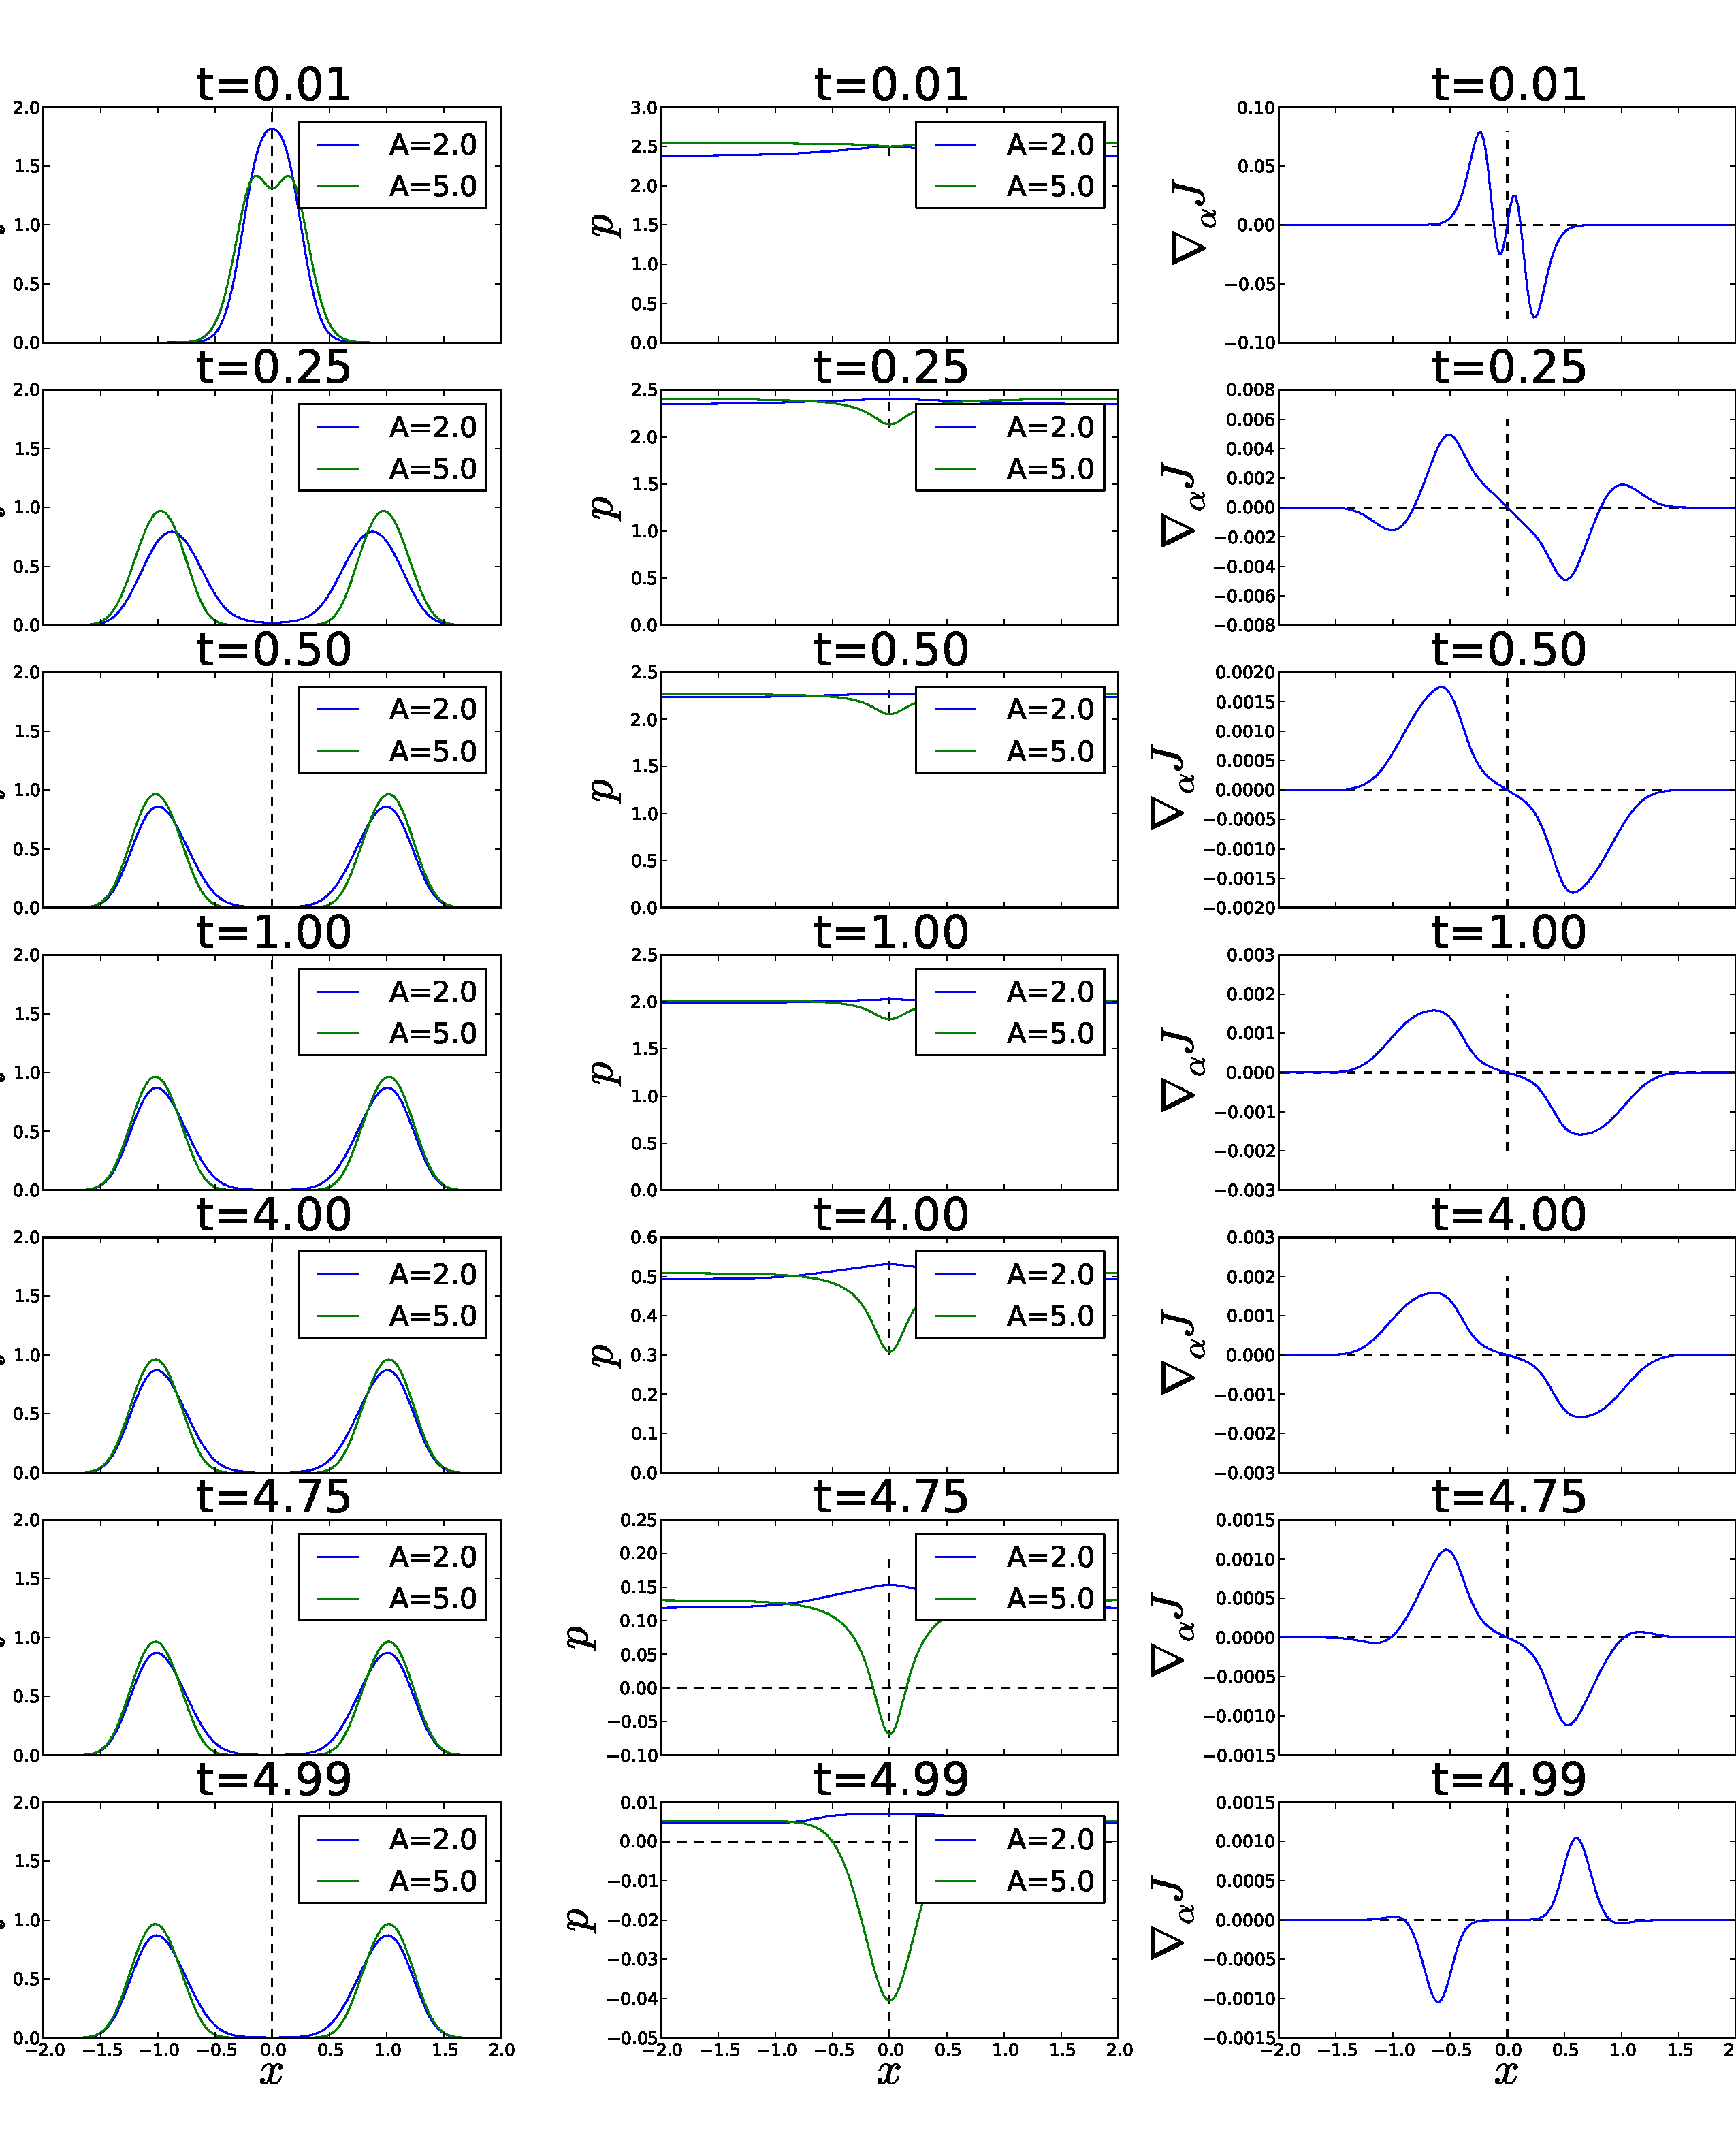
\includegraphics[width=\textwidth]{Figs/DoublewellFBSolver/FB_alpha_null_solution.pdf}
  \caption[labelInTOC]{Solution to the test Double Well potential problem using
  $\a \equiv 0$. On the left, the density $f$, in the middle the adjoint $p$, 
  on the right the gradient $\delta J/ \delta \a$, sampled at different times
<<<<<<< HEAD
  $t=.0, .01, 1.0,\ldots5.0$} 
  \label{fig:FBSoln_doublewell_alpha_null}
\end{center}
\end{figure}

=======
  $t=.0, .01, 1.0,\ldots5.0$}
  \label{fig:FBSoln_doublewell_alpha_null}
\end{center}
\end{figure}
>>>>>>> 6d1ee3c9eb52b6bed66343a6488d0f9a4ca3aef0
 \clearpage

\subsubsection{Going through a full gradient descent iteration}
We start with the simplest possible approach which is just to push the alpha in
the gradient direction $K$ number of times. We see that for $K> 15$, $J$ doesn't
change much and so we stop there. 

The $\a_k$ iterates and the evolution of $J$ are shown in resp.

%\usepackage{graphics} is needed for \includegraphics
\begin{figure}[htp]
\begin{center}
  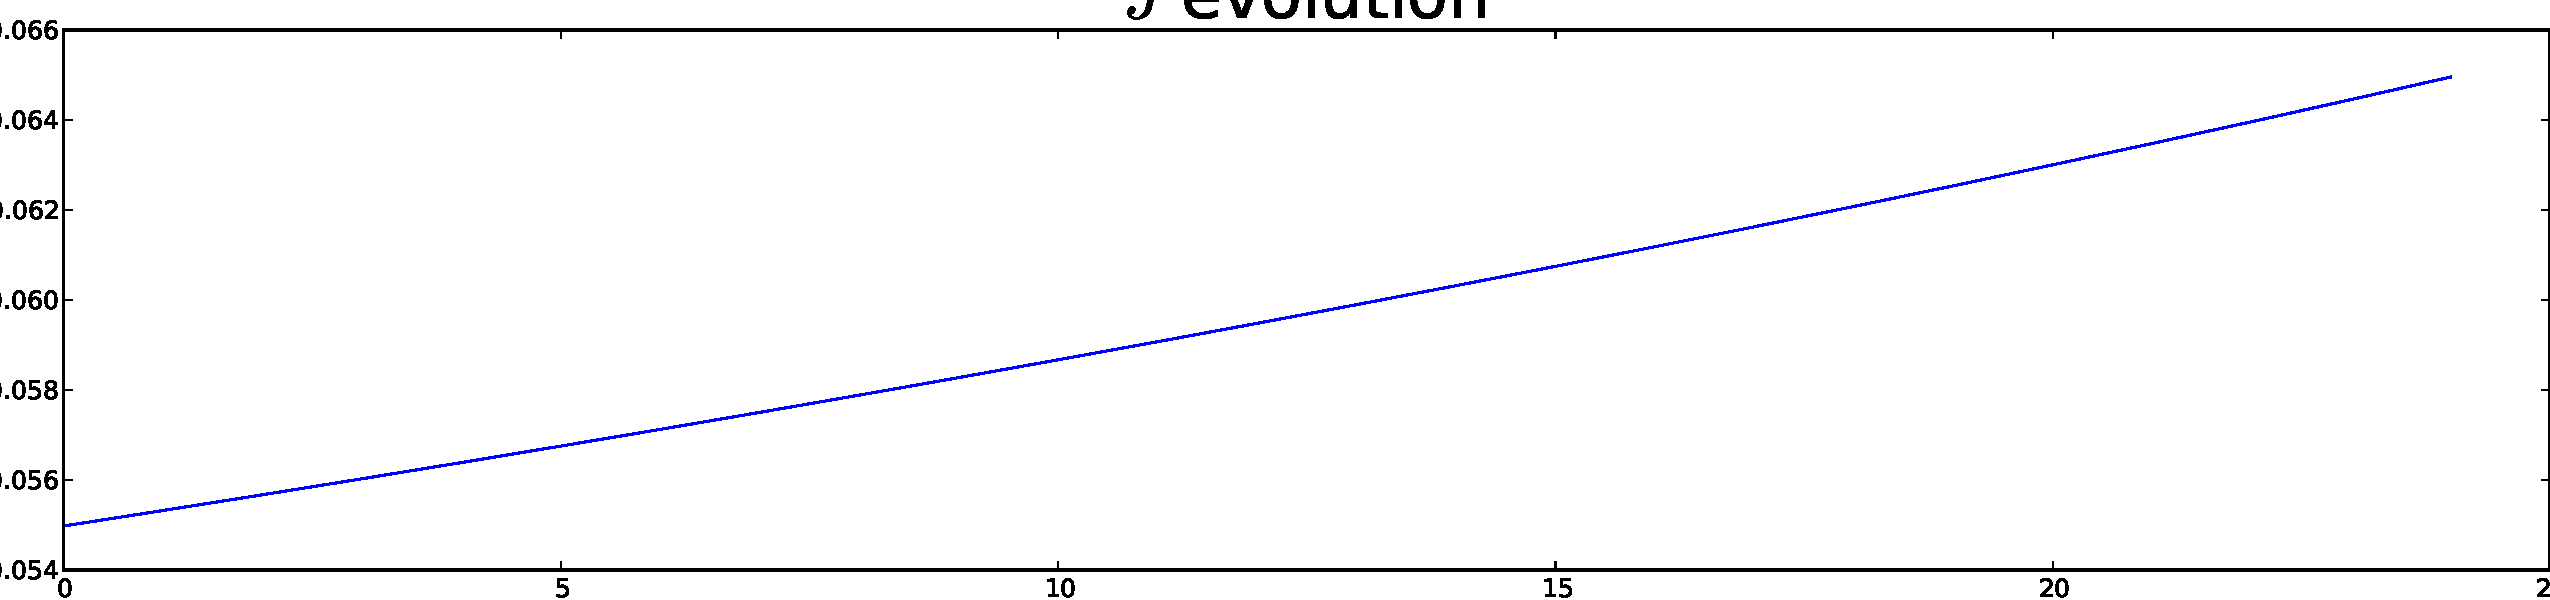
\includegraphics[width=\textwidth]{Figs/DoublewellFBSolver/FB_J_iterates_example.pdf}
  \caption[labelInTOC]{Evolution of $J_k$ during a gradient ascent procedure}
  \label{fig:J_iterates_double_well_example}
\end{center}
\end{figure}

\begin{figure}[htp]  
\begin{center}
  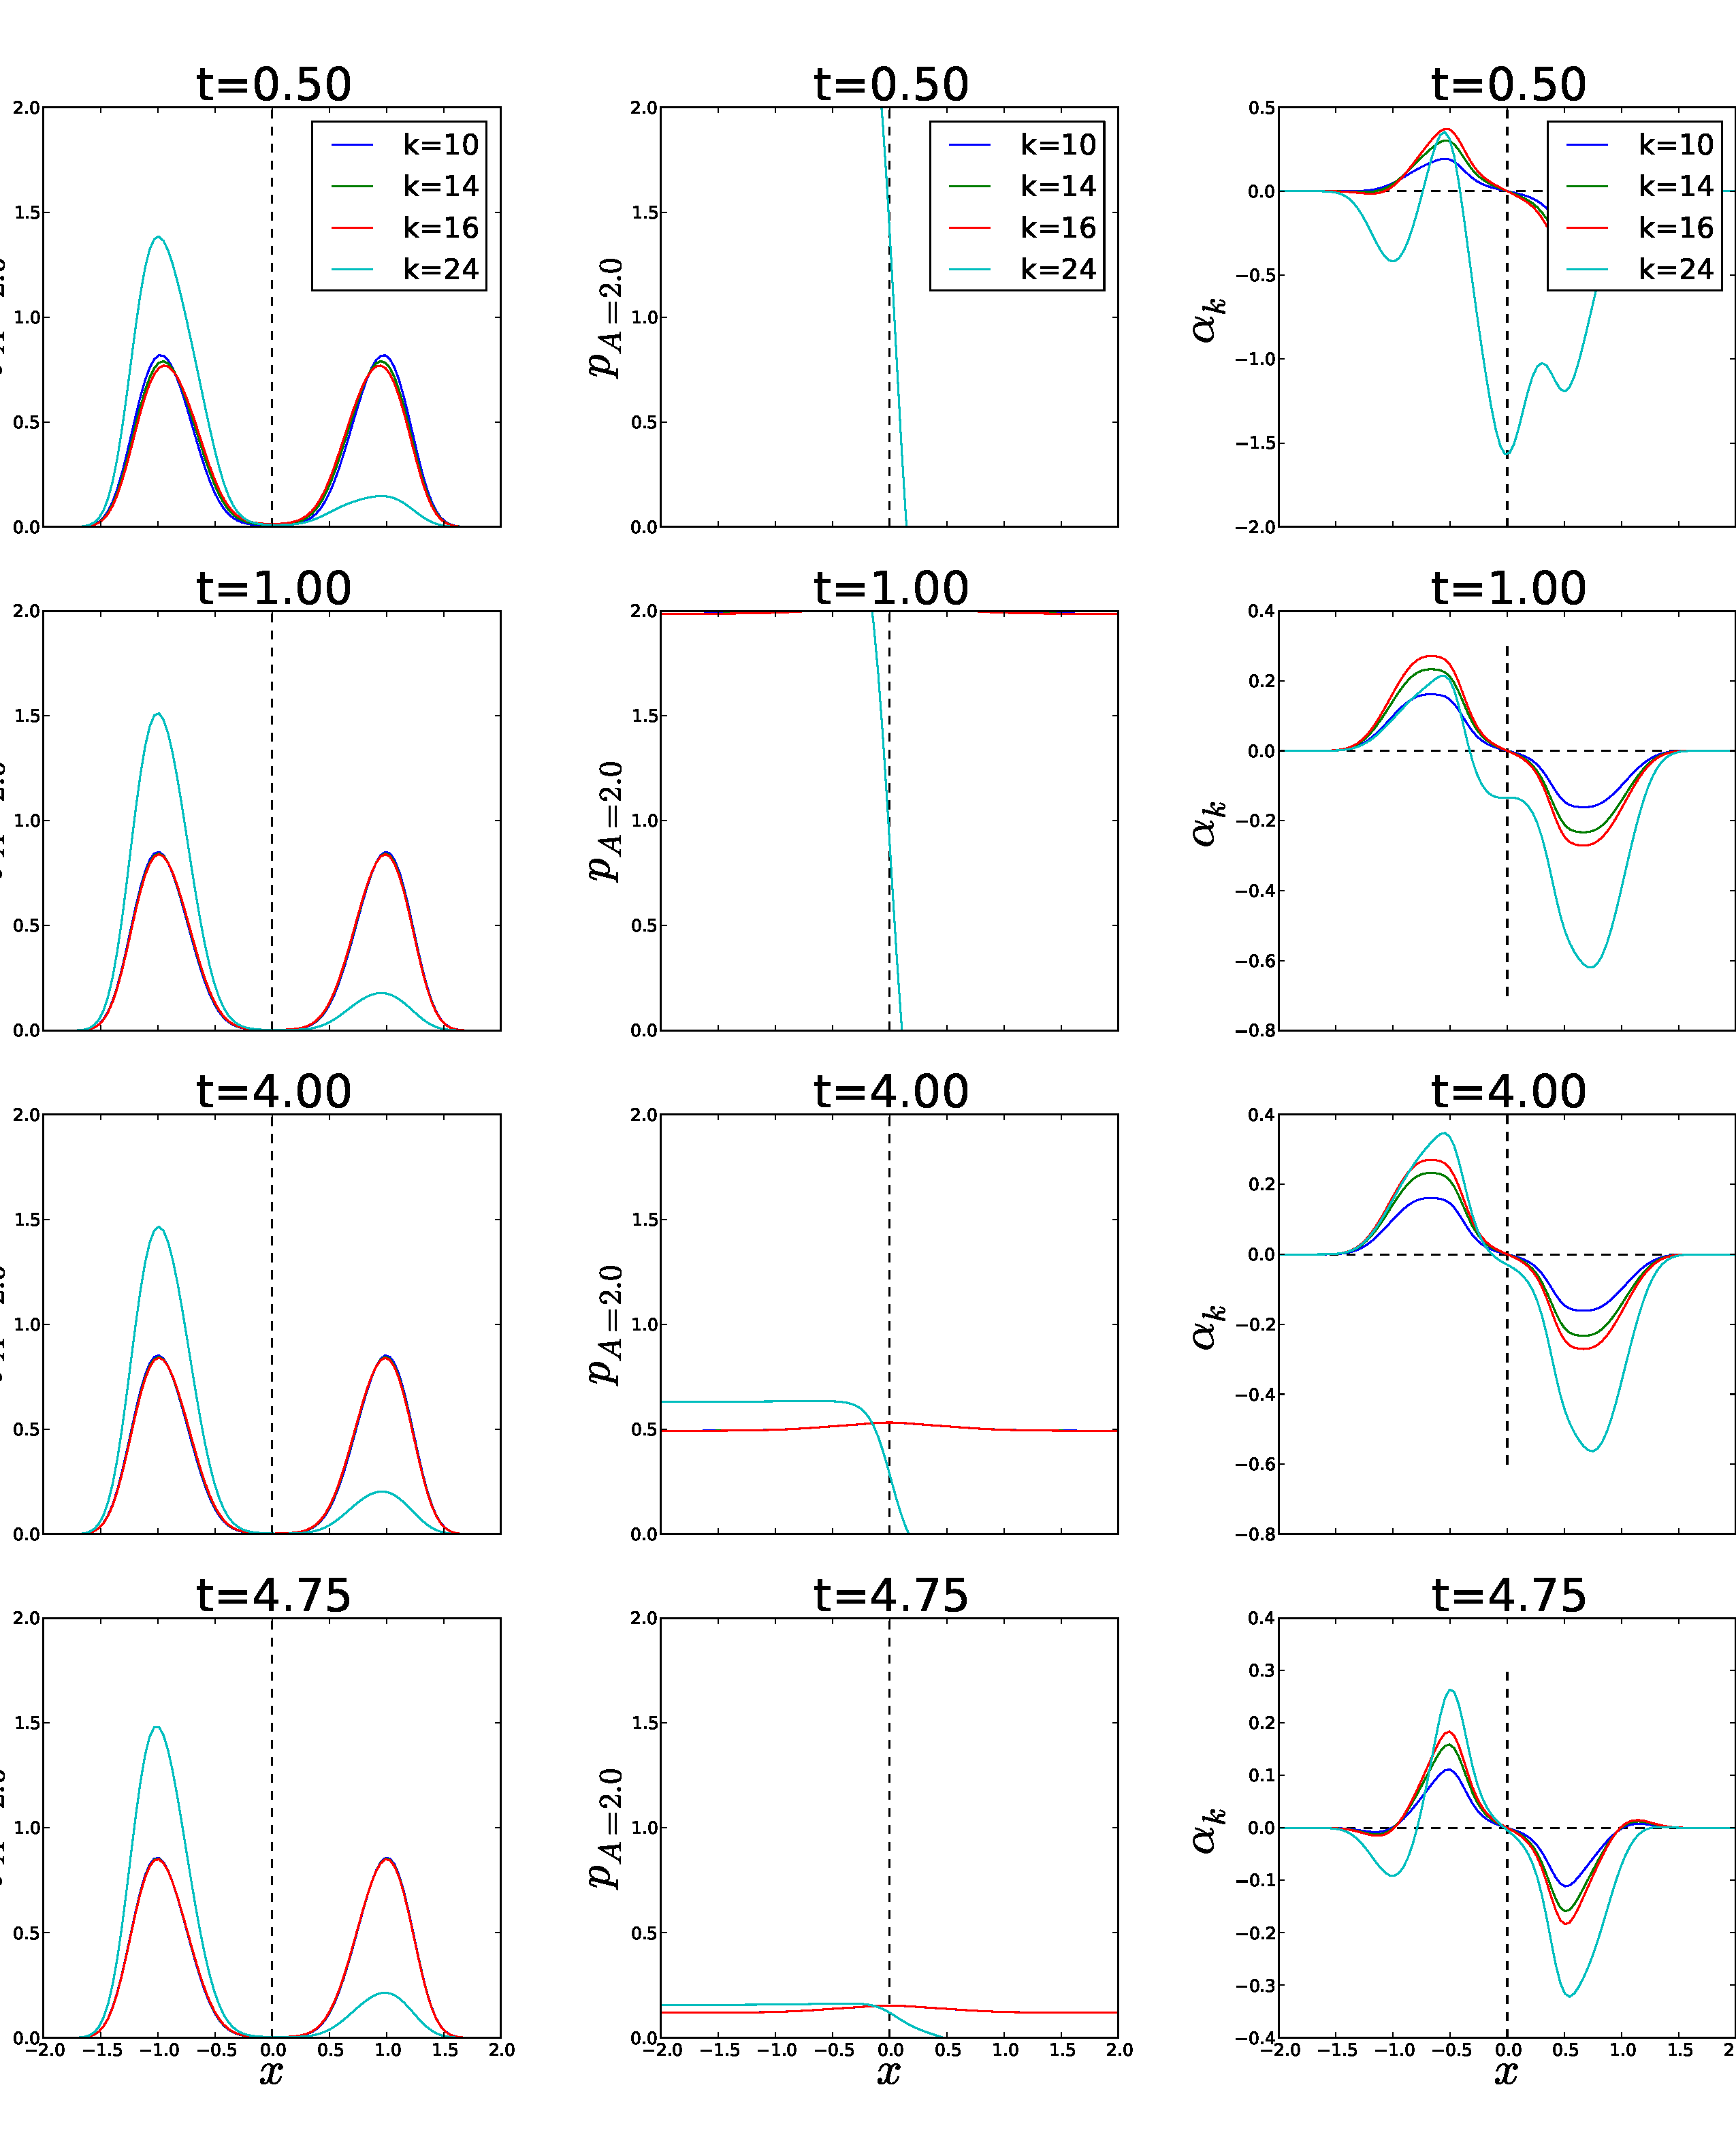
\includegraphics[width=\textwidth]{Figs/DoublewellFBSolver/FB_alpha_iterates_example.pdf}
  \caption[labelInTOC]{Evolution of $\a_k$ during a gradient ascent procedure.
  On the left we show one of the transition densities $f_{A}$ and on the right
  we show the control field for different iterates $k$ in the ascent
  procedure}
  \label{fig:alpha_iterates_double_well_example}
\end{center}
\end{figure}

\clearpage

<<<<<<< HEAD
\subsection{MP Approach - Stationary}
\label{sec:MP_Doublewell_Statinoary}
Unfortunately, we saw that the gradient ascent procedure used in
\cref{sec:MP_Doublewell_TimeDependent} had the tendency to converge to
something 'wrong' (see \cref{fig:alpha_iterates_double_well_example}. 

We now try to see whether restricting ourselves to the statinoary case will make
things better\ldots

Let's explicitly restate the stationarity equations for $\ft,\pt$
\begin{equation}
\begin{gathered}
0 = -\di_x [ U(x;A, \a) \cdot f(x )] + D \di_x^2
f(x )
\\
\begin{array}{ll}
	&
	\left\{ \begin{array}{lcll}
	U f - D \di_x f \big|_{x=\xmin,\xmax} &\equiv& 0 & \textrm{reflecting BCs
	at some } \xmin, \xmax \end{array} \right.
\end{array}
\label{eq:forward_density_double_well_stationary}
\end{gathered}
\end{equation}

\begin{equation}
\begin{gathered}
D \di_x^2 \pt(x ) +
U(x;A, \a(x ))\cdot \di_x p(x ) =
- 1 + \frac{  w_\th \ft }{\sum_\th \wt\ft} 
- \log\left(\frac{f_\th} {\sum_\th \wt \ft }\right)
\\
\begin{array}{ll}
	&
	\left\{ \begin{array}{lcll}
	\di_x \pt(x, t)|_{x = \xmin, \xmax}  &=& 0  \quad &\textrm{BCs}
\end{array} \right.
\end{array}
\label{eq:backward_adjoint_double_well_statinoary}
\end{gathered}
\end{equation}

Having computed $\ft, \pt$, we compute the gradient $\delta J / \delta \a$
as
$$
\frac {\delta J}{\delta \a} |_{x} = \sum_\th \wt (\di_x \pt \cdot \ft)
$$
This just restates \cref{eq:differential_objective_stationary_wrt_control_final}.

\subsubsection{Gradient Ascent for the Stationary-MP}
We start by setting our initial guess $$\a_0(x) \equiv 0$$ 

Again, we would like to see that 
$$ \sgn \left(\frac {\delta J}{\delta \a}\right) \Big|_{x} = - \sgn(x)$$
That is that for negative $x$ we want to drive to the right, $\a > 0$ and for
positive $x$ we want to drive to the right $\a < 0$. 
Let's check.  

The results are visualized in \cref{fig:FBSoln_doublewell_stationary_iterates}. Let's
discuss \cref{fig:FBSoln_doublewell_stationary_iterates}. In general we have
the right tendency, but something is obviously wrong\ldots. All these wiggles
and stuff. In general we cannot get to the bang-bang solution. At least not
using the simple-minded gradient ascent procedure we have implemented so far.  
Although we do have improvement in the objective,
\cref{fig:FBSoln_doublewell_stationary_objective_ascent} with the ascent
procedure, we just can't reach the bang-bang solution\ldots. On the other hand if we were
to try the bang-bang solution, we will find that it is much better than the
gradient ascent optimal. In fact:
$$
J_{\textrm{bang-bang}} =  0.31 \gg 0.09 = J_{\textrm{opt} } 
$$

\begin{figure}[htp]
\begin{center} 
  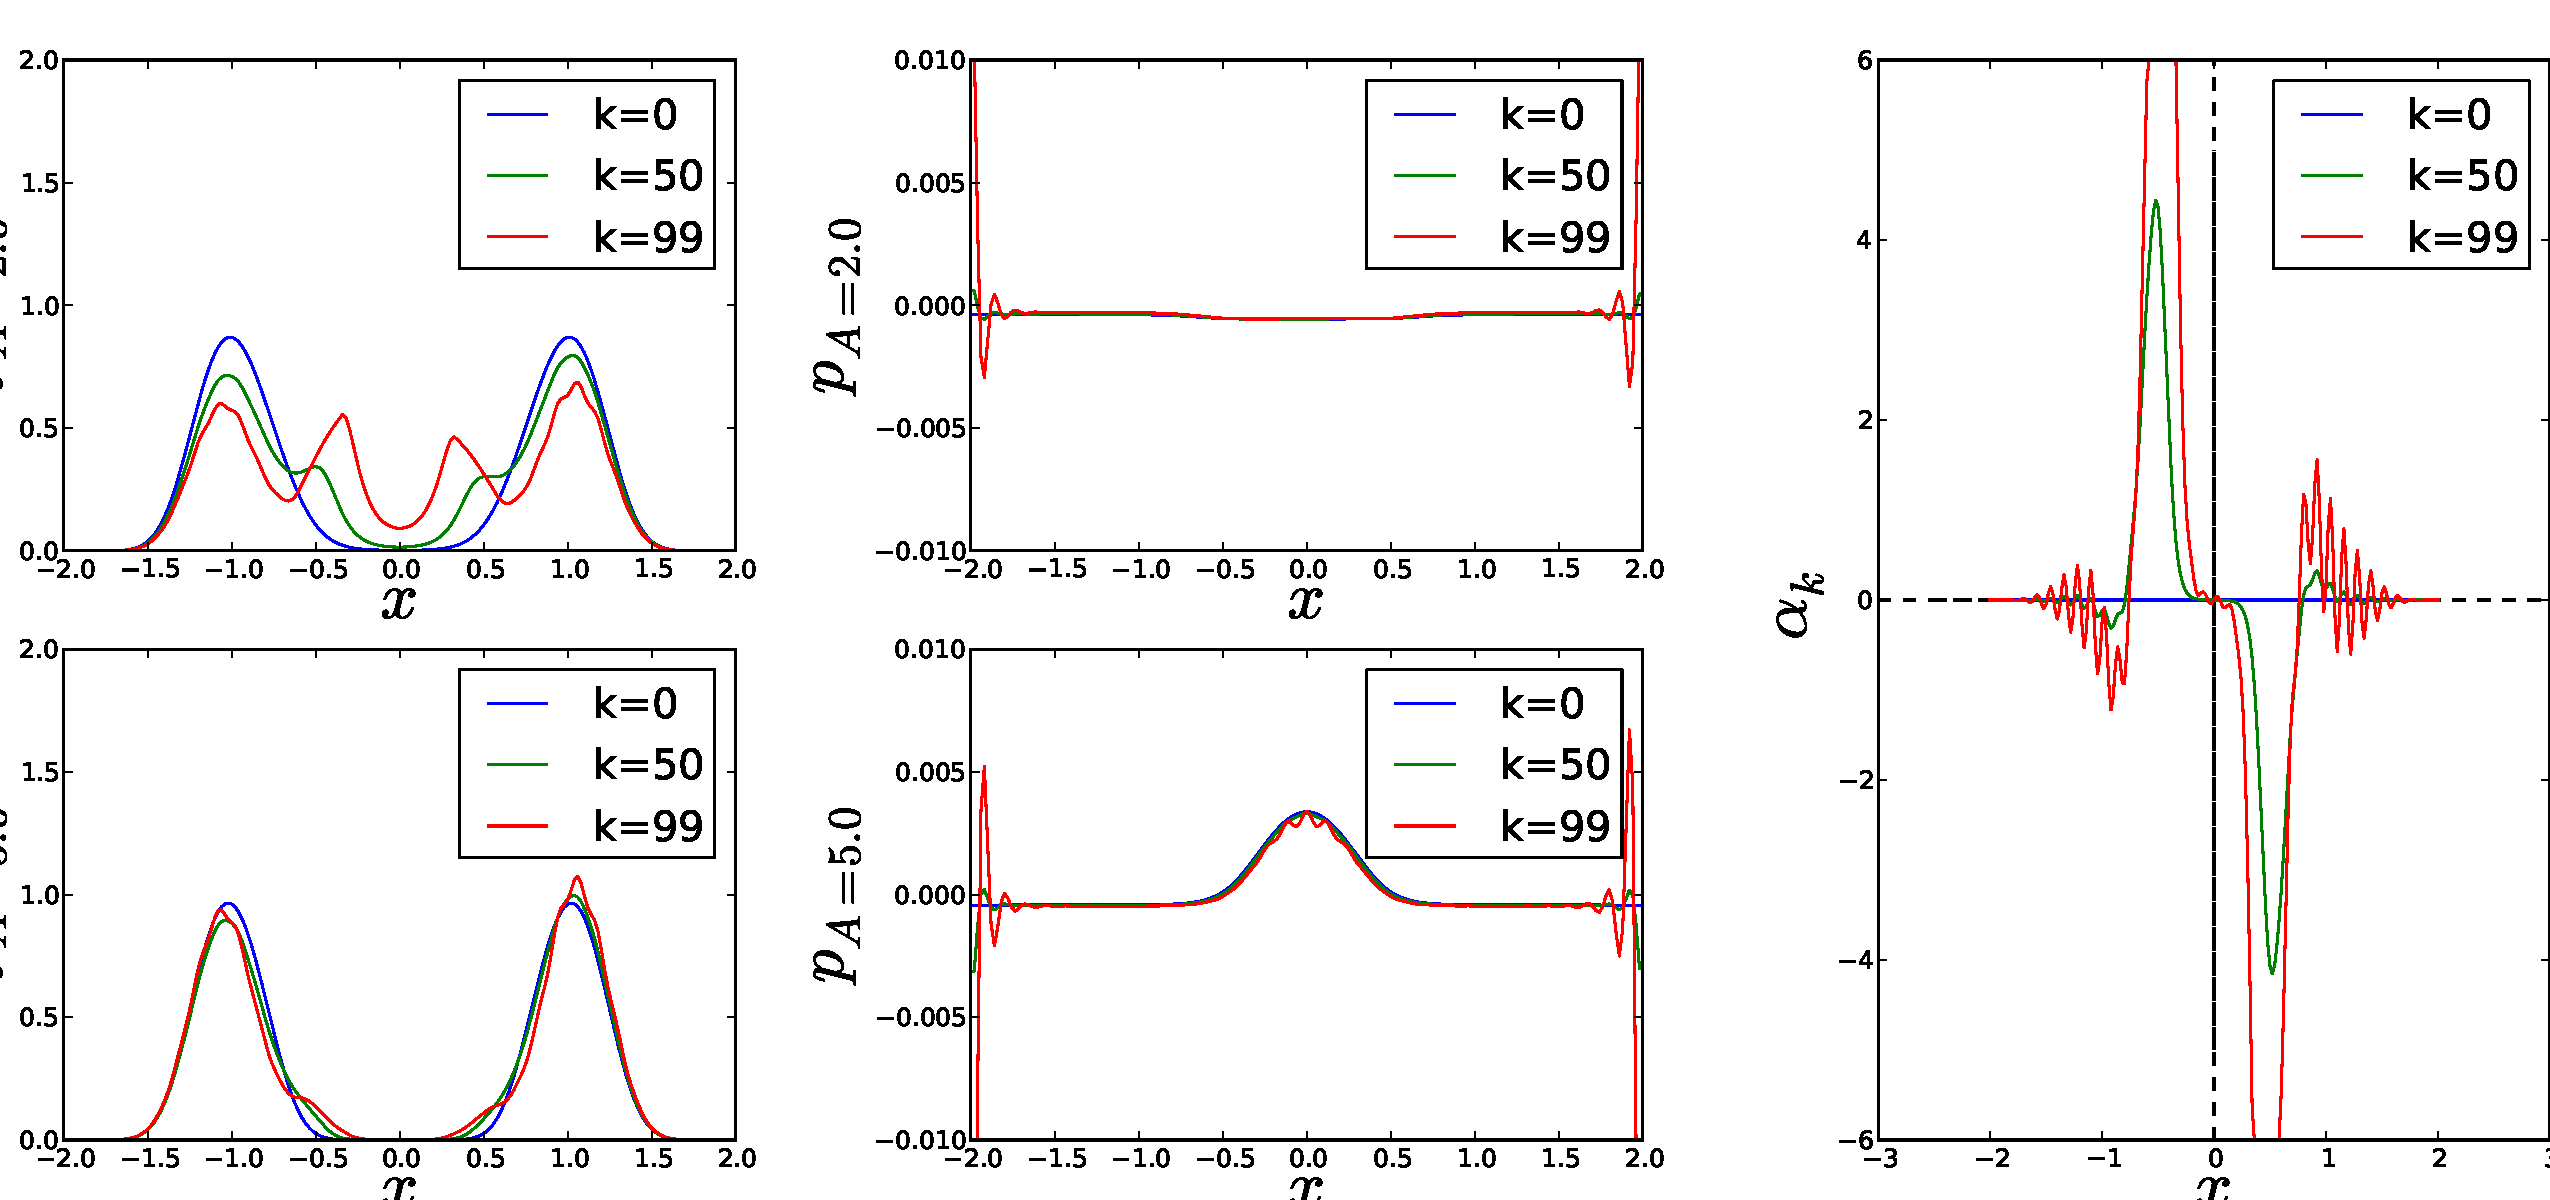
\includegraphics[width=\textwidth]{Figs/DoublewellFBStatinoary/FB_alpha_iterates_example.pdf}
  \caption[labelInTOC]{Gradient Ascent for the stationary Double-Well potential problem starting from $\a \equiv 0$. On the left, the density $\ft(x)$, in the middle
  the adjoint $\pt$, on the right the gradient $\delta J/ \delta \a$}
  \label{fig:FBSoln_doublewell_stationary_iterates}
\end{center}
\end{figure}
 
\begin{figure}[htp]
\begin{center} 
  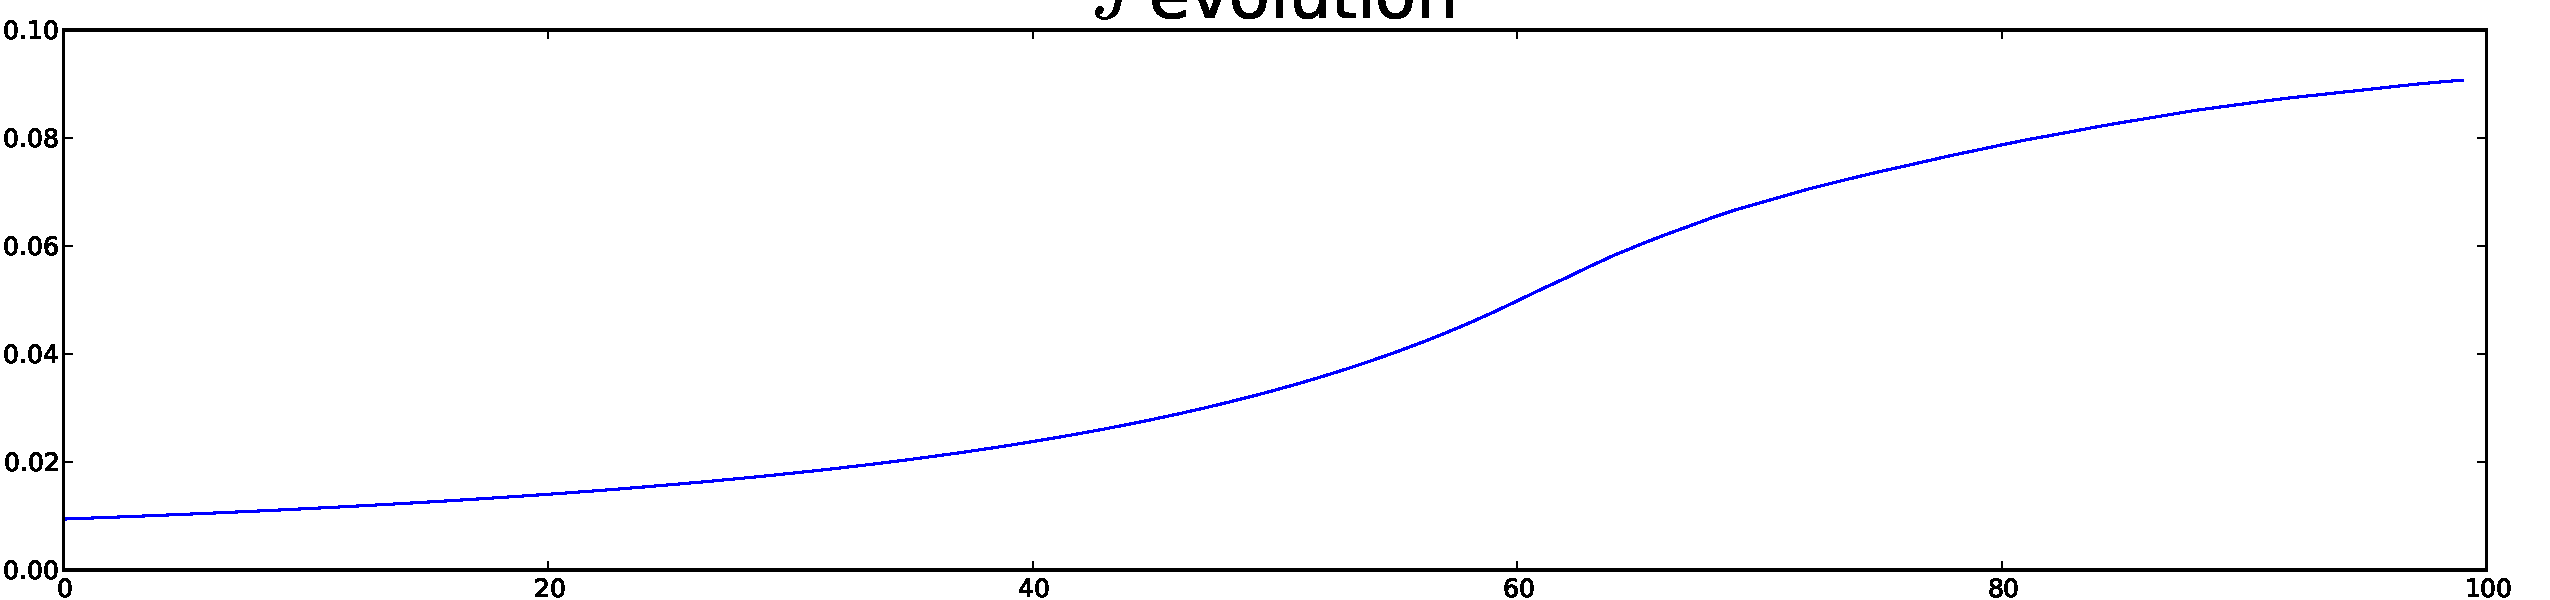
\includegraphics[width=\textwidth]{Figs/DoublewellFBStatinoary/FB_J_iterates_example.pdf}
  \caption[labelInTOC]{Objective Evolution for the Gradient Ascent for the
  stationary Double Well potential problem starting from $\a \equiv 0$.}
  \label{fig:FBSoln_doublewell_stationary_objective_ascent}
\end{center}
\end{figure}

\clearpage
















=======
>>>>>>> 6d1ee3c9eb52b6bed66343a6488d0f9a4ca3aef0

\subsection{DP appraoch}
I DON''T THINK THIS IS FEASBILE - AT LEAST I HAVEN''T FIGURED OUT HOW TO DO IT
YET, SEE \cref{sec:DP_4_OptEstimate} for DISCUSSION OF PROBLEMS.

%  We would now want to follow up the theoretical
% developments
% from
% \cref{sec:DP_4_OptEstimate} with an concrete example.
% 
% Thus our first test problem will be the problem on estimating the double-well
%  potential barrier height as in Sec. 4 of the latest draft of \cite{Lin} on
%  arXiv. (From June 7th, 2013). We shall use exactly the same parameter values
%  etc. as in sec. 4 in \cite{Lin}. 
% 
% Note that our $r$ in \cref{eq:reward_funciont_mutual_information} doesn't depend
% on the chosen value for $\a(x,t)$ (it only depends on their up-to-now history)
% and thus $r$ can be taken outside the maximization wrt.\ $\a$ in
% \cref{eq:HJB_equation_with_prior}.
%  
% However then we are back to the old bang-bang problem, in that if $\a$ appears
% linearly in $U$ then we would want to push it to either of its extreme values.
%  
% Thus we could consider regularizing our control problem by introducing the
% familiar, smoothing, energy-penalty term - $\eps \a^2 / 2$.
% 
% Let me explain in detail.
% 
% Consider \cref{eq:HJB_equation_with_prior}
% $$
% \di_t w(x,t) + \sup_{\a(x,t)} \bigg\{  \Exp_\th \big[\Lstar_\th [w] +
% r(x|\th)\big] \bigg\} = 0
% $$ 
% 
% For the double-well potential, $\Lstar$ is given by:
% $$
% \Lstar_\th[w]  = \underbrace{-\left( x^3 - x + A \frac xc e^{-(x/c)^2} - \a
% \right)}_{U(x,t;\th, \a)} \di_x w + D \di_x^2 w $$
% And the goal is to estimate the barrier height, $A$. I.e.\ 
% $$\th = \{A\}$$
% which is located at $x=0$. All other parameters, $c,D$, are assumed known. 
% 
% Thus when for fixed $x,t$, we seek $\a(x,t)$ which maximizes the expression
% $$
% \Exp_\th \big[\Lstar_\th [w] + r(x|\th)\big]
% $$
% this reduces to maximizing
% $$
% \a(x,t) \di_x w(x,t)
% $$
% And so
% $$
% \a(x,t) = \sgn{[\di_x w(x,t)]} \cdot \amax 
% $$
% 
% All intuition suggests that the sign of the gradient of the value function will
% be the negative of the sign of $x$. I.e.\ that the bang-bang control
% will push the particle to cross the barrier and be positive for negative $x$ and
% vice-versa. We will check if that is true below. 
% 
% How does that relate to the derivations in sec. 4 in \cite{Lin}?
% 
% In \cite{Lin}, they also conclude that the optimal control is bang-bang, except
% in a small neighbourhood of the origin. I.e.\ near the barrier, where $x \approx
% 0$. There the control is attenuated, although it still has a sign that
% nudges the particle towards crossing the barrier, i.e.\ it is positive for
% negative $x$ and vice-versa.
% 
% One explanation why the control is not bang-bang in \cite{Lin} near the location
% of the barrier is the order of discretization/optimization. As far as I can
% tell, they first discretize their system in space-time and only then optimize,
% i.e. choose the controls. For large enough time-steps, it makes sense then to
% attenuate the control just before crossing the barrier, since too strong a
% stimulus will not only help in crossing the barrier, but also subsequently push
% the particle too far away from it, before the next time-step and the next
% control update.
% 
% \subsection{Nitty-gritty computations for the double-well potential}
% We would not like to compute the forward density and the value functions $f, w$
% for the double-well problem in order to verify that indeed the bang-bang control
% is optimal and that the switching point is the origin, i.e.\ the location of the
% barrier. 
% 
% Let's explicitly state the equations for the evolution of the density and
% the value functions, $f,w$
% \begin{equation}
% \begin{gathered}
% \di_t f(x,t; \th, \a(\cdot)) = -\di_x [ U(x; \th, \a) \cdot f(x,t)] + D \di_x^2
% f(x,t)
% \\
% \begin{array}{ll}
% 	& 
% 	\left\{ \begin{array}{lcll}
% 	 f(x,0) &=& \delta(x-x_0)  &\textrm{delta function at some } x_0
% 	\\
% 	U f - D \di_x f \big|_{x=\xmin,\xmax} &\equiv& 0 & \textrm{reflecting BCs
% 	at some } \xmin, \xmax \end{array} \right.
% \end{array}
% \label{eq:forward_density_double_well}
% \end{gathered}
% \end{equation}
% 
% \begin{equation}
% \begin{gathered}
% \di_t w(x,t) +
% D \di_x^2w(x,t) +
% \Exp_\th \big[ U(x; \th, \a(x,t))\cdot \di_x w(x,t) + r(x|\th)\big]= 0,
% \\
% \a (x,t) = \sgn (\di_x w(x,t) )\cdot \amax
% \\
% \begin{array}{ll}
% 	& 
% 	\left\{ \begin{array}{lcll}		
% 	\di_x w(x, t)|_{x = \xmin, \xmax}  &=& 0  \quad &\textrm{reflecting BCs}
% 	\\
% 	w(x,\T)  &=& 0 \,& \textrm{TCs}
% \end{array} \right.
% \end{array}
% \label{eq:value_function_double_well}
% \end{gathered}
% \end{equation}
% 
% where, recall, 
% $$
% U(x,t;\th, \a) = -\left( 4x^3 - 4x -A \frac xc e^{-(x/c)^2/2} \right) + \a(x,t) 
% $$
% and
% $$
% r(x|\th ) = \log\left(\frac{f(x,t | \th )}
% {\int_\th f(x,t|\th) \rho(\th)\intd{\th}}\right)
% $$
% 
% To be explicit about what the effect of the integration wrt.\ the prior $\th$
% is, we can write the evolution part of the HJB equation,
% \cref{eq:value_function_double_well} as
% \begin{eqnarray*}
% -\di_t w(x,t)  =&
% \left( -4x^3 + 4x + \Exp_\th[A] \frac xc e^{-(x/c)^2/2}  + \a(x,t) \right) \di_x
% w(x,t) 
% \\
% &+ D \di_x^2w(x,t)  +
%  \Exp_\th \big[  \log\left(\frac{f(x,t | \th )}
% 				{\int_\th f(x,t|\th) \rho(\th)\intd{\th}}\right) \big] 
% \end{eqnarray*}
% i.e.\ we need to take the average value of $A$ and of the infinitesimal
% mutual information, $r(x|\th)$.
% 
% Following \cite{Lin} (but not exactly) we set the parameters as $\s = 1.
% \implies D = 0.5$,
% % (actually it is a
% % little smaller in \cite{Lin}, but this eases the numerics)
% $c = 0.3$ and $A = 4$ as the true value of $A$ under which the actual process
% will evolve.
% 
% For the prior on $A$ we use a uniform over $[2,5]$, which we represent with
% $N_\th = 10$ uniform points - $[2.0,  2.33, \ldots 5.0]$.
% 
% The forward density must be started at a point - we use $x_0 = 0$, to make our
% life simpler. I.e.\ we assume the process starts at the location of the barrier.
% 
% The control is constrained to lie in the set $[-10, 10]$, i.e.\ $\amax = 10$.
% 
% The space is constrained to $x \in [-5,5]$, i.e.\ $\xmin, \xmax = -5,5$. It is
% further discretized using $\Delta x = .1$, i.e.\ with 101 uniform points, $[-5,
% -4.9\ldots 5.]$.
% 
% We will run the solver until $T = 5$.

<<<<<<< HEAD
\clearpage

\section{Second Illustrative Example - the time-constant for the OU model}
\label{sec:MP_Doublewell_TimeDependent}
We now follow up the theoretical developments from \cref{sec:MP_with_a_prior}
with a concrete example.

Our first test problem will be the problem on estimating the double-well
potential barrier height as in Sec. 4 of the latest draft of \cite{Lin} on
arXiv. (From June 7th, 2013). We shall use exactly the same parameter values
etc. as in sec. 4 in \cite{Lin}.

We would now like to compute the forward density and the adjoint functions
$\{\ft, \pt\}$ for the double-well problem.

Let's explicitly state the evolution equations for $\ft,\pt$
\begin{equation}
\begin{gathered}
\di_t \ft(x,t; \th, \a(\cdot)) = -\di_x [ U(x;A, \a) \cdot \ft(x,t)] + D \di_x^2
\ft(x,t)
\\
\begin{array}{ll}
	&
	\left\{ \begin{array}{lcll}
	 \ft(x,0) &=& \delta(x-x_0)  &\textrm{delta function at some } x_0
	\\
	U \ft - D \di_x \ft \big|_{x=\xmin,\xmax} &\equiv& 0 & \textrm{reflecting BCs
	at some } \xmin, \xmax \end{array} \right.
\end{array}
\label{eq:forward_density_double_well}
\end{gathered}
\end{equation}

\begin{equation}
\begin{gathered}
-\di_t \pt(x,t) =
D \di_x^2 \pt(x,t) +
U(x;A, \a(x,t))\cdot \di_x \pt(x,t) \\
+ 1 - \frac{  w_\th \ft }{\sum_\th \pt_\th\ft} 
+ \log\left(\frac{f_\th} {\sum_\th \wt \ft }\right)
\\
\begin{array}{ll}
	&
	\left\{ \begin{array}{lcll}
	\di_x \pt(x, t)|_{x = \xmin, \xmax}  &=& 0  \quad &\textrm{BCs}
	\\
	\pt(x,\T)  &=& 0 \,& \textrm{TCs}
\end{array} \right.
\end{array}
\label{eq:backward_adjoint_double_well}
\end{gathered}
\end{equation}
where,  
\begin{eqnarray*}
U(x; A, \a) &= -\frac 1 \tc \left( \m -x \right) + \a(x,t)
\\
&= -\grad_x \left(\mathcal V(x) + \mathcal{A}(x) \right)
\end{eqnarray*}

Having computed $\ft, \pt$, we compute the gradient $\delta J / \delta \a$
as
$$
\frac {\delta J}{\delta \a} |_{x,t} = \sum_\th \wt (\di_x \pt \cdot \ft)
$$
This just restates \cref{eq:differential_objective_wrt_control_final}.

For the fixed params we assume $\s = 1. \implies D = 0.5$, $\m = 0$.


For the prior on $\tc$ we use a uniform over $[10,40]$, which we represent with
only $N_\th = 2$ uniform points - $[10, 40]$.  In general, it is
not clear how to start the forward density, i.e., what its ICs should be. 

For now, let's use a delta mass at $x_0 = 0$, i.e.\ we assume the process starts
at the crest of the barrier. The control is constrained to lie in the set $[-10, 10]$, i.e.\ $\amax
= 10$. The space is constrained to $x \in [-2.,2.]$, i.e.\ $\xmin, \xmax =
-2.,2.$, using  It is further discretized using $\Delta x = .1$, i.e.\ with 101
uniform points, $[-5, -4.9\ldots 5.]$.

Let's first see what happens when we run the solver until $T = 5$..

The experiment proceeds as follows: For our initial guess we take $$\a_0(x,t)
\equiv 0$$ Then we would like to see that 
$$ \sgn \left(\frac {\delta J}{\delta \a}\right) \Big|_{x,t} = - \sgn(x)$$
That is that for negative $x$ we want to drive to the right, $\a > 0$ and for
positive $x$ we want to drive to the right $\a < 0$. 
Let's see.  

The results are visualized in \cref{fig:FBSoln_doublewell_alpha_null}. Let's
discuss \cref{fig:FBSoln_doublewell_alpha_null}. The most important plots are on
the right, $\delta J$ which indicate how we are supposed to be changing $\a$. 
It is clear that except for the very beginning $t \approx 0$, and the end $t
\approx T$, $\delta J$ is essentially constant in time.  

Let's focus then on what happens in the bulk of time in the middle. Indeed we  
have that 
$$
\sgn \left(\frac {\delta J}{\delta \a}\right) \Big|_{x,t} = - \sgn(x)
$$
which implies that we should push the particle to the right (resp. left)
depending on whether we are to the left (resp. right) of the barrier at $x=0$.
Everything looks good, except for two points.
\begin{enumerate}
  \item The magnitude of $\delta J$ is very small. If we were to take steps of
  size $s=1.$, it would take us thousands of iteratons to get to what we expect to be
the right solution, i.e. bang-bang at $\amax = 10$.
\item The behaviour of $\delta J$ is 'wrong' or 'surprising near the end, $t
\approx T$, which appear around $t>4.75$ and there is also some discrepancies
near the beginning, the negative wiggles for $t \approx 0$, which vanish by the
time $t > 0.5$
\end{enumerate}

Both issues are minor, but we shall keep them in mind when we go through a full
iteration of the gradient descent. 
%\usepackage{graphics} is needed for \includegraphics
\begin{figure}[htp] 
\begin{center} 
  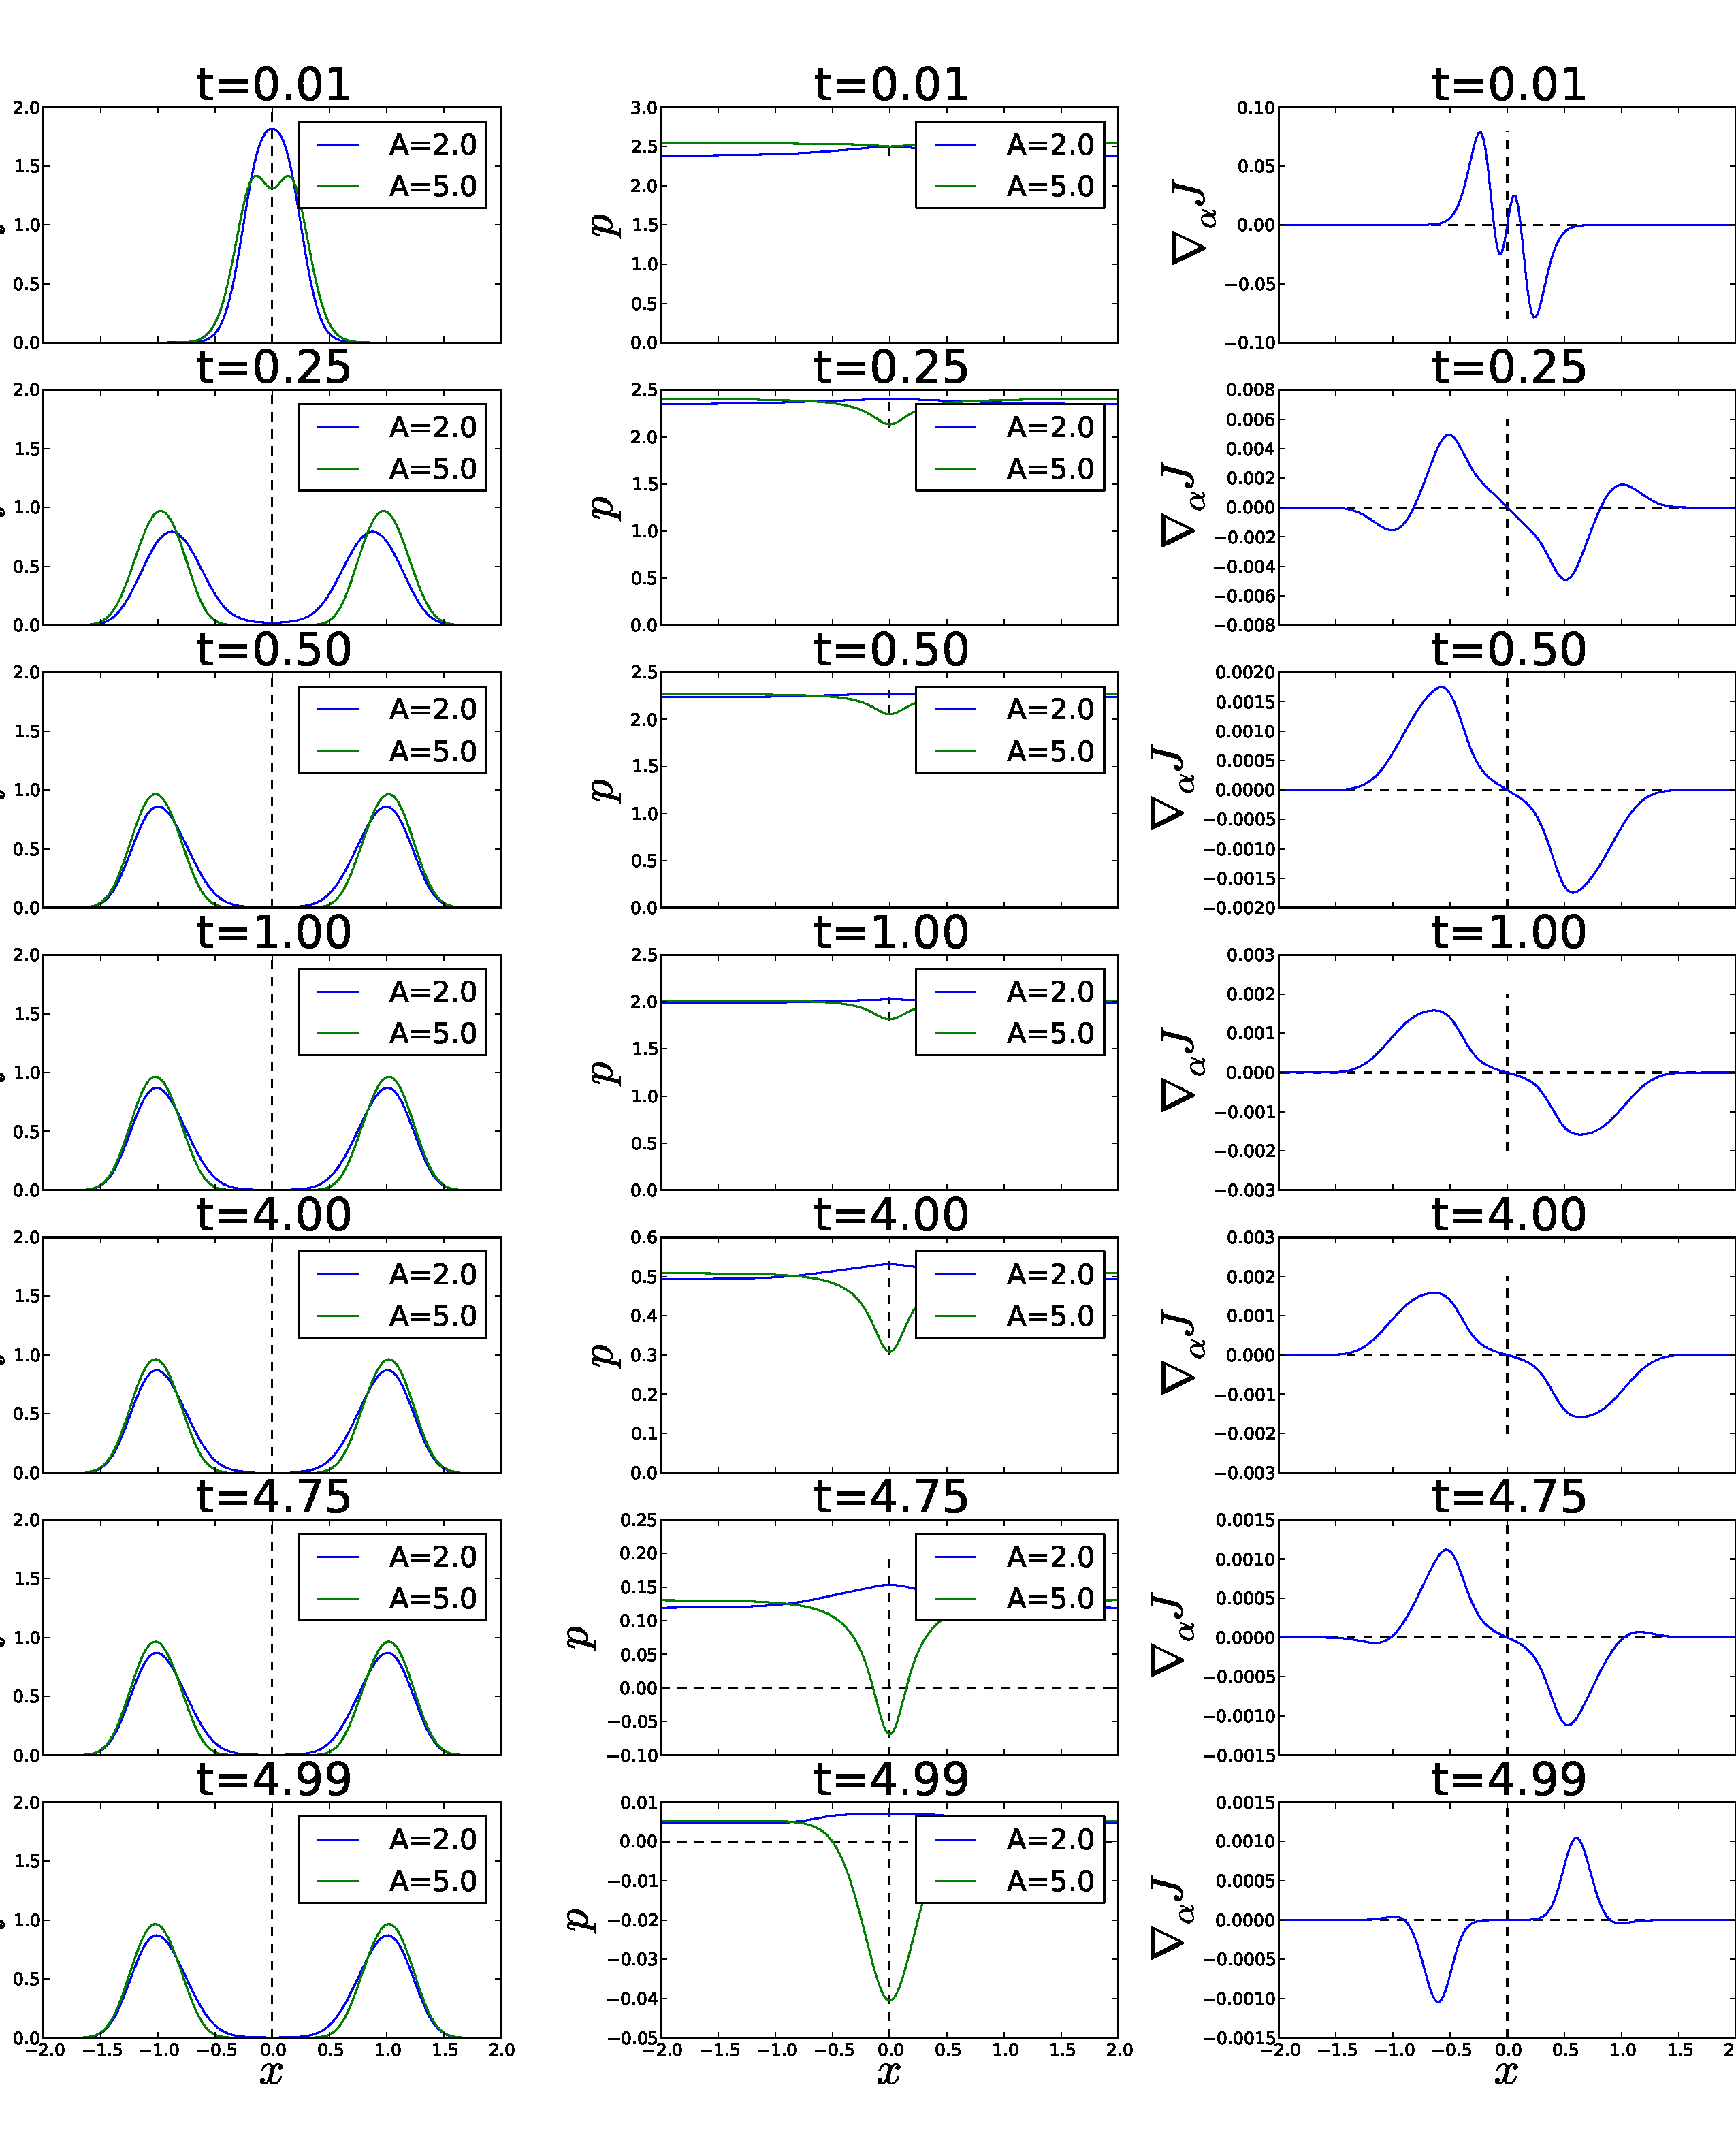
\includegraphics[width=\textwidth]{Figs/DoublewellFBSolver/FB_alpha_null_solution.pdf}
  \caption[labelInTOC]{Solution to the test Double Well potential problem using
  $\a \equiv 0$. On the left, the density $f$, in the middle the adjoint $p$, 
  on the right the gradient $\delta J/ \delta \a$, sampled at different times
  $t=.0, .01, 1.0,\ldots5.0$} 
  \label{fig:FBSoln_doublewell_alpha_null}
\end{center}
\end{figure}

 \clearpage

\subsubsection{Going through a full gradient descent iteration}
We start with the simplest possible approach which is just to push the alpha in
the gradient direction $K$ number of times. We see that for $K> 15$, $J$ doesn't
change much and so we stop there. 

The $\a_k$ iterates and the evolution of $J$ are shown in resp.

%\usepackage{graphics} is needed for \includegraphics
\begin{figure}[htp]
\begin{center}
  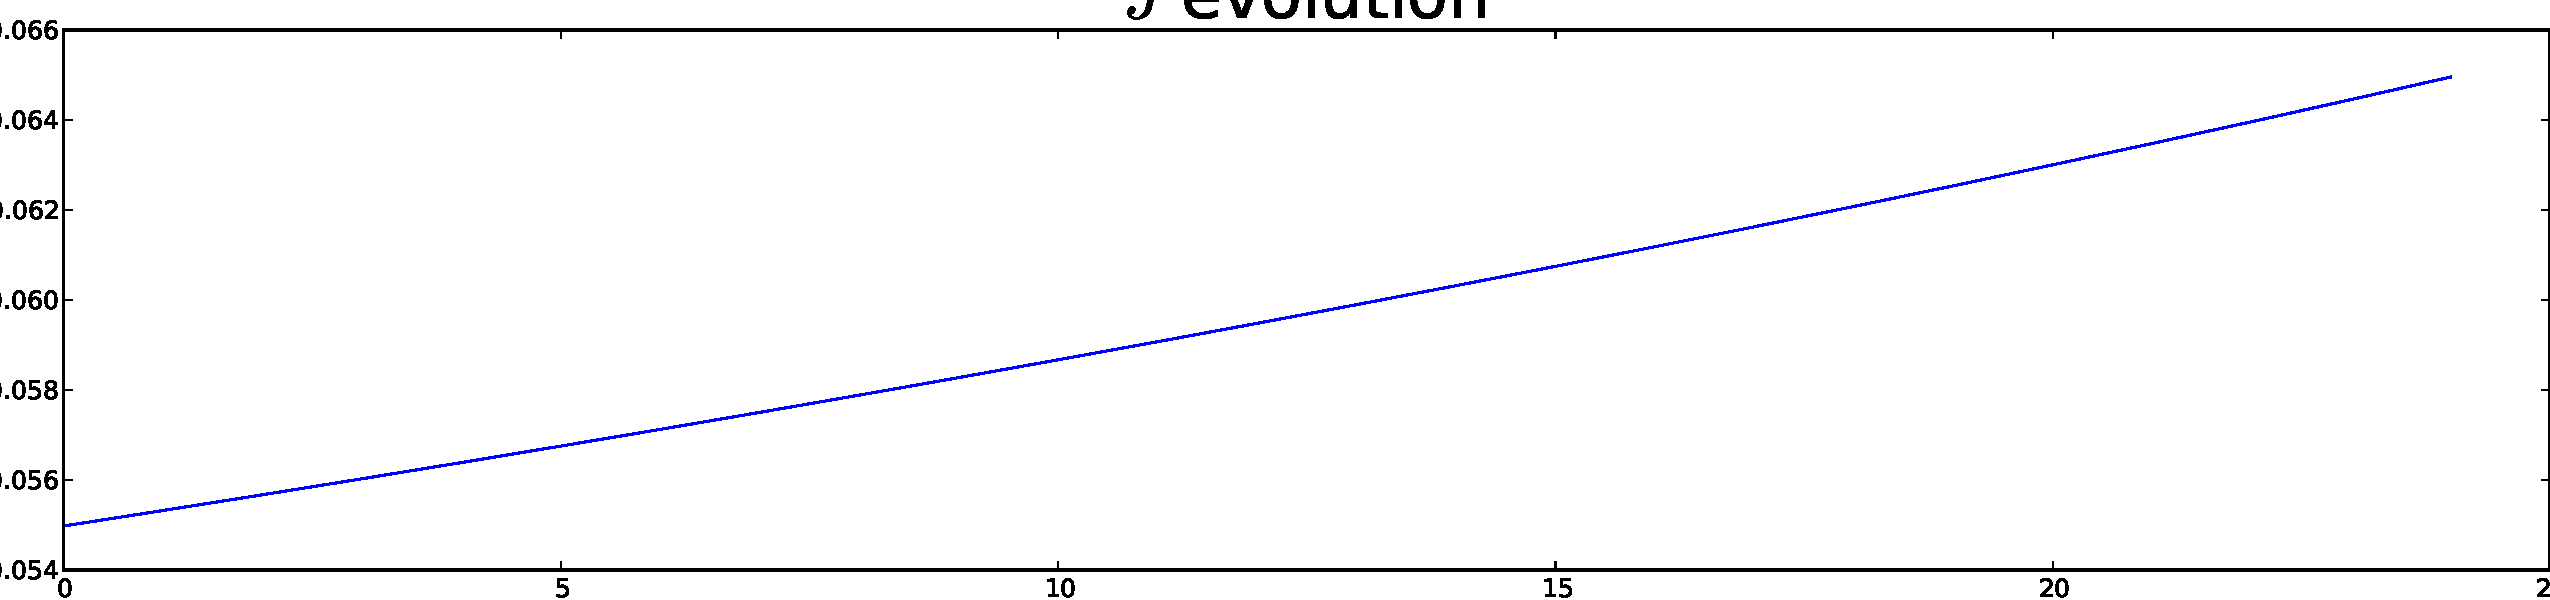
\includegraphics[width=\textwidth]{Figs/DoublewellFBSolver/FB_J_iterates_example.pdf}
  \caption[labelInTOC]{Evolution of $J_k$ during a gradient ascent procedure}
  \label{fig:J_iterates_double_well_example}
\end{center}
\end{figure}

\begin{figure}[htp]  
\begin{center}
  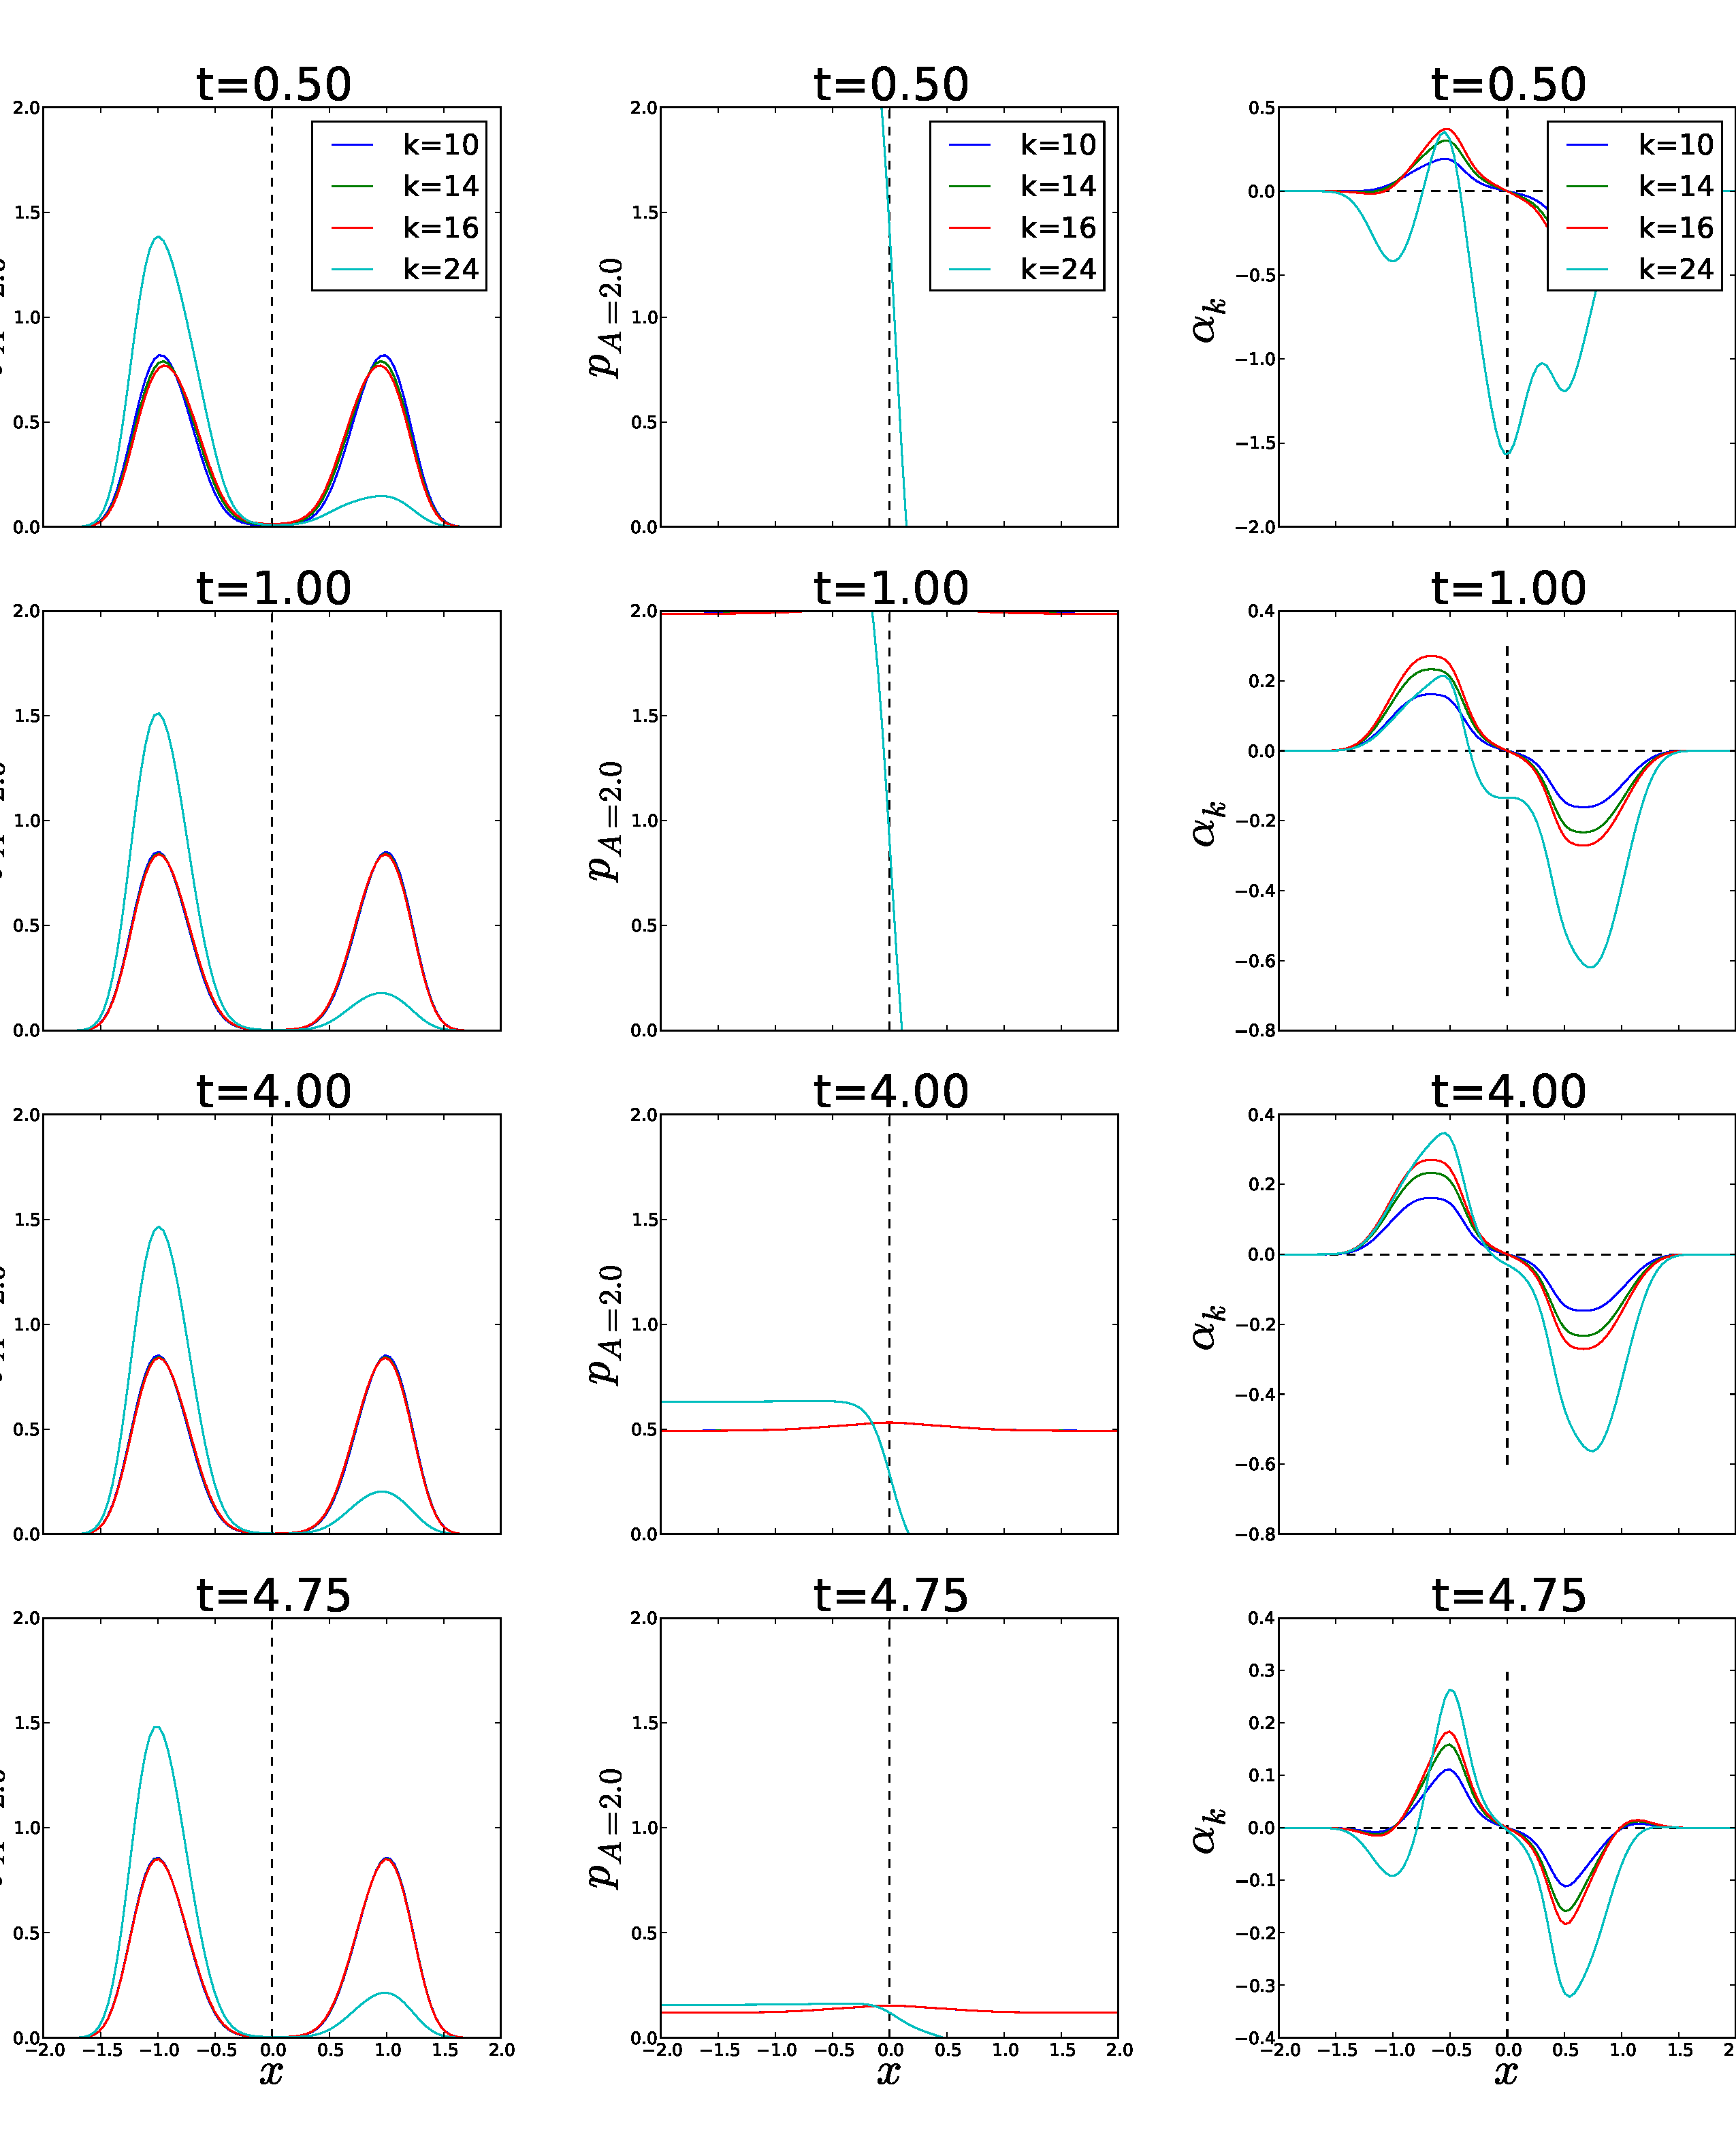
\includegraphics[width=\textwidth]{Figs/DoublewellFBSolver/FB_alpha_iterates_example.pdf}
  \caption[labelInTOC]{Evolution of $\a_k$ during a gradient ascent procedure.
  On the left we show one of the transition densities $f_{A}$ and on the right
  we show the control field for different iterates $k$ in the ascent
  procedure}
  \label{fig:alpha_iterates_double_well_example}
\end{center}
\end{figure}

\clearpage











\clearpage
\appendix
=======

\section{Second Illustrative Example - the time-constant for the OU model}

\clearpage \appendix
>>>>>>> 6d1ee3c9eb52b6bed66343a6488d0f9a4ca3aef0
\section{Mutual Info calculation}
\label{sec:mutual_info_defn} 
Here we show why \cref{eq:mutual_info_with_posterior} for
the Mutual Information agrees with the usual definition of the Mutual Information, which
for the two random variables, $X,\th$ is
\begin{equation}
I(X,\th) = \int_\Theta \int_X p(x,\th) \cdot \log \left(
\frac{p(x,\th)}{p(x)p(\th)}\right) \intd{x} \intd{\th}
\label{eq:mutual_info_defn}
\end{equation}

First of all, $p(\th)$  is just the prior of $\th$, $$p(\th) = \rho(\th)$$.
The joint distribution is $$p(x,y) = L(x|\th)\rho(\th)$$, while the $x$
marginal is $$p(x) = \int_\Theta L(x|\th)\rho(\th) \intd{\th}$$.
Plugging the three expressions into the definition in
\cref{eq:mutual_info_defn} gives:
\begin{equation}
I = \int_\Theta \int_X L(x|\th)\rho(\th) \cdot 
\log \left( \frac{L(x|\th)\rho(\th) }{\int_\Theta L(x|\th)\rho(\th) \intd{\th}
\cdot \rho(\th) } \right)
\intd{x}\intd{\th}.
\label{eq:mutual_info_prior_trajectory}
\end{equation}
And after canceling $\rho(\th)$ inside the $\log$, we get
\cref{eq:mutual_info_with_likelihood} which is equivalent to
\cref{eq:mutual_info_with_posterior}.




\bibliographystyle{plain} 
\bibliography{library,local}

\end{document}